% arara: lualatex
% arara: biber
% arara: makeindex
% arara: makeglossarieslite
% arara: lualatex
% arara: lualatex
% arara: latexmk: { clean: partial }
% arara: clean: { extensions: [bbl, glo, gls, glg, ist, suc, syc] }


%-----------------------------------
% Define document and include general packages
%-----------------------------------
% Tabellen- und Abbildungsverzeichnis stehen normalerweise nicht im
% Inhaltsverzeichnis. Gleiches gilt für das Abkürzungsverzeichnis (siehe unten).
% Manche Dozenten bemängeln das. Die Optionen 'listof=totoc,bibliography=totoc'
% geben das Tabellen- und Abbildungsverzeichnis im Inhaltsverzeichnis (toc=Table
% of Content) aus.
% Da es aber verschiedene Regelungen je nach Dozent geben kann, werden hier
% beide Varianten dargestellt.
\documentclass[12pt,oneside,titlepage,listof=totoc,bibliography=totoc]{scrartcl}% „oneside“ mit „twoside“ austauschen um beidseitigen Druck zu ermöglichen
%TC:ignore
%\documentclass[12pt,oneside,titlepage]{scrartcl}

%-----------------------------------
% Dokumentensprache
%-----------------------------------
%\def\FOMEN{}% Auskommentieren um die Dokumentensprache auf englisch zu ändern


%-----------------------------------
% Meta informationen
%-----------------------------------
%-----------------------------------
% Meta Informationen zur Arbeit
%-----------------------------------

% Autor
\newcommand{\myAutor}{Joshua-Volkan Gramatzki}


% Titel der Arbeit
\newcommand{\myTitel}{Auswirkungen von Zero Trust Network Security zur Bekämpfung moderner Cyberbedrohungen}


% Betreuer
\newcommand{\myBetreuer}{Prof. Dr. Gregor Hülsken}


% Lehrveranstaltung
\newcommand{\myLehrveranstaltung}{IT-Infrastruktur}


% Matrikelnummer
\newcommand{\myMatrikelNr}{647100}


% Ort
\newcommand{\myOrt}{Ahaus}


% Datum der Abgabe
\newcommand{\myAbgabeDatum}{\today}


% Semesterzahl
\newcommand{\mySemesterZahl}{3}


% Name der Hochschule
\newcommand{\myHochschulName}{FOM Hochschule für Oekonomie \& Management}


% Standort der Hochschule
\newcommand{\myHochschulStandort}{Münster}


% Studiengang
\newcommand{\myStudiengang}{Wirtschaftsinformatik}


% Art der Arbeit
\newcommand{\myThesisArt}{Seminararbeit}


% Zu erlangender akademische Grad
\newcommand{\myAkademischerGrad}{Bachelor of Science (B.Sc.)}


% Firma
\newcommand{\myFirma}{Tobit Software Laboratories AG}

% Forschungsfrage
\newcommand{\myForschungsfrage}{Wie trägt eine \ac{zta} zur Erhöhung der Sicherheit in einem System unter Einbehalt von Benutzerfreundlichkeit und -produktivität bei?}





\usepackage[ngerman]{babel}
\usepackage[utf8]{luainputenc}
\usepackage[utf8]{inputenc}
\usepackage[babel,german=quotes]{csquotes}
\usepackage{fancyhdr}
\usepackage{fancybox}
\usepackage[a4paper, left=4cm, right=2cm, top=4cm, bottom=2cm]{geometry}
\usepackage{graphicx}
\usepackage{colortbl}
\usepackage[capposition=bottom]{floatrow}
\usepackage{array}
\usepackage{float}      %Positionierung von Abb. und Tabellen mit [H] erzwingen
\usepackage{footnote}
\usepackage{booktabs}
\usepackage{epigraph}


\usepackage{pgfplots}
\usepackage{pgfplotstable}
\pgfplotsset{compat = 1.17}

% Darstellung der Beschriftung von Tabellen und Abbildungen (Leitfaden S. 44)
% singlelinecheck=false: macht die Caption linksbündig (statt zentriert)
% labelfont auf fett: (Tabelle x.y:, Abbildung: x.y)
% font auf fett: eigentliche Bezeichnung der Abbildung oder Tabelle
% Fettschrift laut Leitfaden 2018 S. 45
\usepackage[labelfont=bf, font=bf, format=hang, justification=justified]{caption}
\usepackage{enumitem}
\usepackage{mathptmx}
% \usepackage{minted} %Kann für schöneres Syntax Highlighting genutzt werden. ACHTUNG: Python muss installiert sein.
\usepackage[scaled=0.9]{helvet} % Behebt, zusammen mit Package courier, pixelige Überschriften. Ist, zusammen mit mathptx, dem times-Package vorzuziehen. Details: https://latex-kurs.de/fragen/schriftarten/Times_New_Roman.html
\usepackage{courier}
\usepackage{amsmath}
\usepackage{amssymb}
%\usepackage[table]{xcolor}
\usepackage{marvosym}            % Verwendung von Symbolen, z.B. perfektes Eurozeichen

\renewcommand\familydefault{\sfdefault}
\usepackage{ragged2e}

% Mehrere Fussnoten nacheinander mit Komma separiert
\usepackage[hang,multiple]{footmisc}
\setlength{\footnotemargin}{1em}

% todo Aufgaben als Kommentare verfassen für verschiedene Editoren
\usepackage{todonotes}

% Verhindert, dass nur eine Zeile auf der nächsten Seite steht
\setlength{\marginparwidth}{2cm}
\usepackage[all]{nowidow}

%-----------------------------------
% Farbdefinitionen
%-----------------------------------
\definecolor{darkblack}{rgb}{0,0,0}
\definecolor{dunkelgrau}{rgb}{0.8,0.8,0.8}
\definecolor{hellgrau}{rgb}{0.0,0.7,0.99}
\definecolor{mauve}{rgb}{0.58,0,0.82}
\definecolor{dkgreen}{rgb}{0,0.6,0}

%-----------------------------------
% Pakete für Tabellen
%-----------------------------------
\usepackage{epstopdf}
\usepackage{nicefrac} % Brüche
\usepackage{multirow}
\usepackage{rotating} % vertikal schreiben
\usepackage{mdwlist}
\usepackage{tabularx}% für Breitenangabe

%-----------------------------------
% sauber formatierter Quelltext
%-----------------------------------
\usepackage{listings}
% JavaScript als Sprache definieren:
\lstdefinelanguage{JavaScript}{
    keywords={break, super, case, extends, switch, catch, finally, for, const, function, try, continue, if, typeof, debugger, var, default, in, void, delete, instanceof, while, do, new, with, else, return, yield, enum, let, await},
    keywordstyle=\color{blue}\bfseries,
    ndkeywords={class, export, boolean, throw, implements, import, this, interface, package, private, protected, public, static},
    ndkeywordstyle=\color{darkgray}\bfseries,
    identifierstyle=\color{black},
    sensitive=false,
    comment=[l]{//},
    morecomment=[s]{/*}{*/},
    commentstyle=\color{purple}\ttfamily,
    stringstyle=\color{red}\ttfamily,
    morestring=[b]',
    morestring=[b]"
}

\lstset{
%language=JavaScript,
    numbers=left,
    numberstyle=\tiny,
    numbersep=5pt,
    breaklines=true,
    showstringspaces=false,
    frame=l ,
    xleftmargin=5pt,
    xrightmargin=5pt,
    basicstyle=\ttfamily\scriptsize,
    stepnumber=1,
    keywordstyle=\color{blue},          % keyword style
    commentstyle=\color{dkgreen},       % comment style
    stringstyle=\color{mauve}         % string literal style
}

%-----------------------------------
%Literaturverzeichnis Einstellungen
%-----------------------------------

% Biblatex

\usepackage{url}
\urlstyle{same}

%%% Neuer Leitfaden (2018) Chicago
\usepackage[
    backend=biber,
    style=ext-authoryear-ibid, % Auskommentieren und nächste Zeile einkommentieren, falls "Ebd." (ebenda) nicht für sich-wiederholende Fussnoten genutzt werden soll.
% style=ext-authoryear,
    maxcitenames=3,    % mindestens 3 Namen ausgeben bevor et. al. kommt
    maxbibnames=999,
    mergedate=false,
    date=iso,
    seconds=true, %werden nicht verwendet, so werden aber Warnungen unterdrückt.
    urldate=iso,
    innamebeforetitle,
    dashed=false,
    autocite=footnote,
    doi=false,
    useprefix=true, % 'von' im Namen beachten (beim Anzeigen)
    mincrossrefs = 1,
    language = german
]{biblatex}%iso dateformat für YYYY-MM-DD

%%%% weitere Anpassungen für BibLaTex
%! suppress = NonMatchingIf
\usepackage{xpatch}


\setlength{\bibhang}{1cm}


%%% Weitere Optionen
%\boolitem[false]{citexref} %Wenn incollection, inbook, inproceedings genutzt wird nicht den zugehörigen parent auch in Literaturverzeichnis aufnehmen

%Aufräumen die Felder werden laut Leitfaden nicht benötigt.
\AtEveryBibitem{%
    \ifentrytype{book}{ \clearfield{issn}%
    \clearfield{doi}%
    \clearfield{isbn}%
    \clearfield{url} \clearfield{eprint} }{} \ifentrytype{collection}{ \clearfield{issn}%
    \clearfield{doi}%
    \clearfield{isbn}%
    \clearfield{url} \clearfield{eprint} }{} \ifentrytype{incollection}{ \clearfield{issn}%
    \clearfield{doi}%
    \clearfield{isbn}%
    \clearfield{url} \clearfield{eprint} }{} \ifentrytype{article}{ \clearfield{issn}%
    \clearfield{doi}%
    \clearfield{isbn}%
    \clearfield{url} \clearfield{eprint} }{} \ifentrytype{inproceedings}{ \clearfield{issn}%
    \clearfield{doi}%
    \clearfield{isbn}%
    \clearfield{url} \clearfield{eprint} }{} }

\renewcommand*{\finentrypunct}{}%Kein Punkt am ende des Literaturverzeichnisses

\renewcommand*{\newunitpunct}{\addcomma\space}
\DeclareDelimFormat[bib,biblist]{nametitledelim}{\addcolon\space}
\DeclareDelimFormat{titleyeardelim}{\newunitpunct}
%Namen kursiv schreiben
\renewcommand*{\mkbibnamefamily}{\mkbibemph}
\renewcommand*{\mkbibnamegiven}{\mkbibemph}
\renewcommand*{\mkbibnamesuffix}{\mkbibemph}
\renewcommand*{\mkbibnameprefix}{\mkbibemph}


% Die Trennung mehrerer Autorennamen erfolgt durch Kommata.
% siehe Beispiele im Leitfaden S. 16
% Die folgende Zeile würde mit Semikolon trennen
%\DeclareDelimFormat{multinamedelim}{\addsemicolon\addspace}

%Delimiter für mehrere und letzten Namen gleich setzen
\DeclareDelimAlias{finalnamedelim}{multinamedelim}

\DeclareNameAlias{default}{family-given} \DeclareNameAlias{sortname}{default} %Nach Namen sortieren

\DeclareFieldFormat{editortype}{\mkbibparens{#1}} \DeclareDelimFormat{editortypedelim}{\addspace}
\DeclareFieldFormat{translatortype}{\mkbibparens{#1}} \DeclareDelimFormat{translatortypedelim}{\addspace}
\DeclareDelimFormat[bib,biblist]{innametitledelim}{\addcomma\space}

\DeclareFieldFormat*{citetitle}{#1} \DeclareFieldFormat*{title}{#1}
\DeclareFieldFormat*{booktitle}{#1} \DeclareFieldFormat*{journaltitle}{#1}

\xpatchbibdriver{online}
{\usebibmacro{organization+location+date}\newunit\newblock} {} {}{}

\DeclareFieldFormat[online]{date}{\mkbibparens{#1}} \DeclareFieldFormat{urltime}{\addspace #1\addspace Uhr}
\DeclareFieldFormat{urldate}{%urltime zu urldate hinzufügen
    [Zugriff\addcolon\addspace #1\printfield{urltime}] } \DeclareFieldFormat[online]{url}{<\url{#1}>}
\renewbibmacro*{url+urldate}{%
    \usebibmacro{url}%
    \ifentrytype{online} {\setunit*{\addspace}%
    \iffieldundef{year} {\printtext[date]{keine Datumsangabe}} {\usebibmacro{date}}}%
    {}%
    \setunit*{\addspace}%
    \usebibmacro{urldate} }

%Verhindern, dass bei mehreren Quellen des gleichen Autors im gleichen Jahr
%Buchstaben nach der Jahreszahl angezeigt werden wenn sich das Keyword in usera unterscheidet.
\DeclareExtradate{ \scope{ \field{labelyear} \field{year} } \scope{ \field{usera} } }

%% Anzeige des Jahres nach dem Stichwort (usera) im Literaturverzeichnis
%% Wenn das Jahr bei Online-Quellen nicht explizit angegeben wurde, wird nach
%% dem Stichwort 'o. J.' ausgegeben. Nach der URL steht dann 'keine
%% Datumsangabe'. Ist das Jahr definiert, wird es an beiden Stellen ausgegeben.
%% Das Zugriffsdatum (urldate) spielt hier keine Rolle.
%% Für Nicht-Online-Quellen wird nichts geändert.
\renewbibmacro*{date+extradate}{%
    \printtext[parens]{%
        \printfield{usera}%
        \setunit{\printdelim{titleyeardelim}}%
        \ifentrytype{online} {\setunit*{\addspace\addcomma\addspace}%
        \iffieldundef{year} {\bibstring{nodate}} {\printlabeldateextra}}%
        {\printlabeldateextra}}}

%% Anzeige des Jahres nach dem Stichwort (usera) in der Fussnote
%% das Stichwort hat der Aufrufer hier schon ausgegeben.
%% siehe auch Kommentar zu: \renewbibmacro*{date+extradate}
\renewbibmacro*{cite:labeldate+extradate}{%
    \ifentrytype{online} {\setunit*{\addspace\addcomma\addspace}%
    \iffieldundef{year} {\bibstring{nodate}} {\printlabeldateextra}}%
    {\printlabeldateextra}}

\DefineBibliographyStrings{german}{ nodate = {{}o.\adddot\addspace J\adddot}, andothers = {et\addabbrvspace al\adddot}, ibidem = {ebd\adddot} }
\DefineBibliographyStrings{english}{ nodate = {{}n.\adddot\addspace d\adddot}, andothers = {et\addabbrvspace al\adddot} }
\DeclareSourcemap{ \maps[datatype=bibtex]{ \map{ \step[notfield=translator, final] \step[notfield=editor, final] \step[fieldset=author, fieldvalue={{{o\noexpand\adddot\addspace V\noexpand\adddot}}}] } \map{ \pernottype{online} \step[fieldset=location, fieldvalue={o\noexpand\adddot\addspace O\noexpand\adddot}] } } }

\renewbibmacro*{cite}{%
    \iffieldundef{shorthand} {\ifthenelse{\ifnameundef{labelname}\OR\iffieldundef{labelyear}} {\usebibmacro{cite:label}%
    \setunit{\printdelim{nonametitledelim}}} {\printnames{labelname}%
    \setunit{\printdelim{nametitledelim}}}%
    \printfield{usera}%
    \setunit{\printdelim{titleyeardelim}}%
    \usebibmacro{cite:labeldate+extradate}} {\usebibmacro{cite:shorthand}}}

\renewcommand*{\jourvoldelim}{\addcomma\addspace}% Trennung zwischen journalname und Volume. Sonst Space; Laut Leitfaden richtig
%Aufgrund der Änderung bzgl des Issues 169 in der thesis_main.tex musste ich die Zeile auskommentieren. Konnte aber das Verhalten, dass die Fußnoten grün sind, im nachhinein nicht feststellen.
%\hypersetup{hidelinks} %sonst sind Fußnoten grün. Dadurch werden Links allerdings nicht mehr farbig dargestellt

\renewbibmacro*{journal+issuetitle}{%
    \usebibmacro{journal}%
    \setunit*{\jourvoldelim}%
    \iffieldundef{series} {} {\setunit*{\jourserdelim}%
    \printfield{series}%
    \setunit{\servoldelim}}%
    \iffieldundef{volume} {} {\printfield{volume}} \iffieldundef{labelyear} {} { (\thefield{year}) %Ansonsten wird wenn kein Volume angegeben ist ein Komma vorangestellt
    } \setunit*{\addcomma\addspace Nr\adddot\addspace} \printfield{number} \iffieldundef{eid} {} {\printfield{eid}} }

% Postnote ist der Text in der zweiten eckigen Klammer bei einem Zitat
% wenn es keinen solchen Eintrag gibt, dann auch nicht ausgeben, z.B. 'o. S.'
% Wenn man das will, kann man das 'o. S.' ja explizit angeben. Andernfalls steht
% sonst auch bei Webseiten 'o. S.' da, was laut Leitfaden nicht ok ist.
\renewbibmacro*{postnote}{%
    \setunit{\postnotedelim}%
    \iffieldundef{postnote} {} %{\printtext{o.S\adddot}}
    {\printfield{postnote}}}

% Abstand bei Änderung Anfangsbuchstabe ca. 1.5 Zeilen
\setlength{\bibinitsep}{0.75cm}


% nur in den Zitaten/Fussnoten den Vornamen abkürzen (nicht im
% Literaturverzeichnis)

\DeclareDelimFormat{nonameyeardelim}{\addcomma\space} \DeclareDelimFormat{nameyeardelim}{\addcomma\space}

\renewbibmacro*{cite}{%
    \iffieldundef{shorthand} {\ifthenelse{\ifciteibid\AND\NOT\iffirstonpage} {\usebibmacro{cite:ibid}} {\printtext[bibhyperref]{\ifthenelse{\ifnameundef{labelname}\OR\iffieldundef{labelyear}} {\usebibmacro{cite:label}%
    \setunit{\printdelim{nonameyeardelim}}} {\toggletrue{abx@bool@giveninits}%
    \printnames[family-given]{labelname}%
    \setunit{\printdelim{nameyeardelim}}}%
    \printfield{usera}%
    \setunit{\printdelim{titleyeardelim}}%
    \usebibmacro{cite:labeldate+extradate}}}} {\usebibmacro{cite:shorthand}}}

%% Definiert @Standard Eintrag
\DeclareBibliographyDriver{standard}{%
    \usebibmacro{bibindex}%
    \usebibmacro{begentry}%
    \usebibmacro{author}%
    \setunit{\labelnamepunct}\newblock
    \usebibmacro{title}%
    \newunit\newblock
    \printfield{number}%
    \setunit{\addspace}\newblock
    \printfield[parens]{type}%
    \newunit\newblock
    \usebibmacro{location+date}%
    \newunit\newblock
    \iftoggle{bbx:url}
    {\usebibmacro{url+urldate}}
    {}%
    \newunit\newblock
    \usebibmacro{addendum+pubstate}%
    \setunit{\bibpagerefpunct}\newblock
    \usebibmacro{pageref}%
    \newunit\newblock
    \usebibmacro{related}%
    \usebibmacro{finentry}}


% Custom Filters
\defbibfilter{standards}{
    \type{standard} or
    \type{patent}
}



\DefineBibliographyStrings{german}{ibidem = {ebd\adddot}}

%  %%%%% IEEE
% \usepackage[
%  backend=biber,
%  style = apa,
%  maxcitenames=3,	% mindestens 3 Namen ausgeben bevor et. al. kommt
%  maxbibnames=999,
%  date=iso,
%  dateera = astronomical,
%  seconds=true, %werden nicht verwendet, so werden aber Warnungen unterdrückt.
%  urldate=iso,
%  backref = true,
%  backrefstyle = three,
%  datecirca = true,
%  dashed=false,
%  autocite=footnote,
%  language = german,
%  sortcites,
%  useprefix=true, % 'von' im Namen beachten (beim Anzeigen)
%  mincrossrefs = 1,
%  defernumbers = true
%  ]{biblatex}%iso dateformat für YYYY-MM-DD

%% et al. anstatt u. a. bei mehr als drei Autoren.
\DefineBibliographyStrings{ngerman}{
    andothers = {{et\,al\adddot}},
}
\DefineBibliographyStrings{english}{
    andothers = {{et\,al\adddot}},
}


%%%%% Alter Leitfaden. Ggf. Einkommentieren und Bereich hierüber auskommentieren
%\usepackage[
%backend=biber,
%style=numeric,
%citestyle=authoryear,
%url=false,
%isbn=false,
%notetype=footonly,
%hyperref=false,
%sortlocale=de]{biblatex}

%weitere Anpassungen für BibLaTex
%%! suppress = NonMatchingIf
% Opptionen für Biblatex
\ExecuteBibliographyOptions{%
giveninits=false, isbn=true, url=true, doi=false, eprint=false, maxbibnames=7, % Alle Autoren (kein et al.)
maxcitenames=2, % et al. ab dem 3. Autor
backref=false, % Rückverweise auf Zitatseiten
bibencoding=utf8, % wenn .bib in utf8, sonst ascii
bibwarn=true, % Warnung bei fehlerhafter bib-Datei
}%

% et al. an Stelle von u.a.
\DefineBibliographyStrings{ngerman}{ andothers = {{et\,al\adddot}}, }

% Klammern um das Jahr in der Fußnote
\renewbibmacro*{cite:labelyear+extrayear}{%
\iffieldundef{labelyear} {} {\printtext[bibhyperref]{%
\mkbibparens{%
\printfield{labelyear}%
\printfield{extrayear}}}}}

\renewbibmacro*{cite:title}{%
\printtext[bibhyperref]{%
\printfield[citetitle]{labeltitle}%
\setunit{\addcomma\space}%
\printdate}}

\DeclareNameFormat{last-first}{%
\iffirstinits {\usebibmacro{name:family-given} {\namepartfamily} {\namepartgiveni} {\namepartprefix} {\namepartsuffix} } {\usebibmacro{name:family-given} {\namepartfamily} {\namepartgiven} {\namepartprefix} {\namepartsuffix} }%
\usebibmacro{name:andothers}}

% Alternative Notation der Fußnoten
% Zeigt sowohl den Nachnamen als auch den Vornamen an
% Beispiel: \fullfootcite[Vgl. ][Seite 5]{Tanenbaum.2003}
\DeclareCiteCommand{\fullfootcite}[\mkbibfootnote] {\usebibmacro{prenote}} {\usebibmacro{citeindex}%
\printnames[sortname][1-1]{author}%
\addspace (\printfield{year})} {\addsemicolon\space} {\usebibmacro{postnote}}

%Autoren (Nachname, Vorname)
\DeclareNameAlias{default}{family-given}

%Reihenfolge von publisher, year, address verändern
% Achtung, bisher nur für den Typ @book definiert

%% Definiert @Book Eintrag
\DeclareBibliographyDriver{book}{%
\printnames{author}%
\newunit\addcolon\space \printfield{title}%
\setunit*{,\space}%
\printfield{edition}%
\setunit*{\addcomma\space}%
\printlist{publisher}%
\newunit\newblockpunct \printlist{location}%
\setunit*{\space}%
\printfield{year}%
\setunit*{,\space}%
\printfield{isbn}%
\finentry}

%% Definiert @Online Eintrag
\DeclareBibliographyDriver{online}{%
\printnames{author}%
\newunit\newblockpunct \printfield{title}%
\setunit*{,\space}%


%\newunit\newblock
\printfield{url}%
\setunit*{,\space Erscheinungsjahr:\space}%
\printfield{year}%
\setunit*{,\space Aufruf am:\space}%
\printfield{note}%
\finentry}

%% Definiert @Article Eintrag
\DeclareBibliographyDriver{article}{%
\printnames{author}%
\newunit\newblockpunct \printfield{title}%
\setunit*{.\space In:\space}%


%\newunit\newblock
\usebibmacro{journal}%
\setunit*{\space (}%
\printfield{year}\newunit{)}%
\finentry}

%% Definiert @Standard Eintrag
\DeclareBibliographyDriver{standard}{%
  \usebibmacro{bibindex}%
  \usebibmacro{begentry}%
  \usebibmacro{author}%
  \setunit{\labelnamepunct}\newblock
  \usebibmacro{title}%
  \newunit\newblock
  \printfield{number}%
  \setunit{\addspace}\newblock
  \printfield[parens]{type}%
  \newunit\newblock
  \usebibmacro{location+date}%
  \newunit\newblock
  \iftoggle{bbx:url}
    {\usebibmacro{url+urldate}}
    {}%
  \newunit\newblock
  \usebibmacro{addendum+pubstate}%
  \setunit{\bibpagerefpunct}\newblock
  \usebibmacro{pageref}%
  \newunit\newblock
  \usebibmacro{related}%
  \usebibmacro{finentry}}

%% Definiert @InProceedings Eintrag
\DeclareBibliographyDriver{inproceedings}{%
\printnames{author}%
\setunit*{,\space (}%
\printfield{year}\newunit{)}%
\newunit\newblockpunct \printfield{title}%
\setunit*{\space}%
\usebibmacro{booktitle}%
\setunit*{,\space}%
\printfield{isbn}%
\setunit*{,\space}%
\printfield{doi}%
\finentry}

%Doppelpunkt nach dem letzten Autor
\renewcommand*{\labelnamepunct}{\addcolon\addspace }


%Komma anstelle des Punktes
\renewcommand*{\newunitpunct}{\addcomma\space}


%Autoren durch Semikolon trennen
\newcommand*{\bibmultinamedelim}{\addsemicolon\space}%
\newcommand*{\bibfinalnamedelim}{\addsemicolon\space}%
\AtBeginBibliography{%
\let\multinamedelim\bibmultinamedelim \let\finalnamedelim\bibfinalnamedelim }

%Titel nicht kursiv anzeigen
\DeclareFieldFormat{title}{#1\isdot}

% Custom Filters
\defbibfilter{standards}{
        type = standard or 
        type = patent
}

%%%% Ende Alter Leitfaden

%Bib-Datei einbinden
\addbibresource{src/literatur/literatur.bib}

% Zeilenabstand im Literaturverzeichnis ist Einzeilig
% siehe Leitfaden S. 14
\AtBeginBibliography{\singlespacing}

%-----------------------------------
% Silbentrennung
%-----------------------------------
\usepackage{hyphsubst}
\HyphSubstIfExists{ngerman-x-latest}{%
    \HyphSubstLet{ngerman}{ngerman-x-latest}}{}

%-----------------------------------
% Pfad fuer Abbildungen
%-----------------------------------
\graphicspath{{./}{./src/abbildungen/}}

%-----------------------------------
% Weitere Ebene einfügen
%-----------------------------------
\usepackage{titletoc}


\makeatletter

% Setze die Tiefe des Inhaltsverzeichnis auf 4 Ebenen
% Damit erscheinen \paragraph-Sektionen auch im Inhaltsverzeichnis
\setcounter{secnumdepth}{4}
\setcounter{tocdepth}{4}


% Fuege Abstand nach unten wie in einer normalen \section hinzu
% Andernfalls haette \paragraph keinen Zeilenumbruch
% Der Zeilenumbruch koennte mit einer leeren \mbox{} ersetzt werden
% Jedoch klebt dann der Text relativ nah an der Ueberschrift
\renewcommand{\paragraph}{%
\@startsection{paragraph}{4}%
{\z@}{3.25ex \@plus 1ex \@minus .2ex}{1.5ex plus 0.2ex}%
{\normalfont\normalsize\bfseries\sffamily}%
}


\makeatother

%-----------------------------------
% Paket für die Nutzung von Anhängen
%-----------------------------------
\usepackage{appendix}

\DeclareMathOperator{\ggd}{ggd}

%-----------------------------------
% Zeilenabstand 1,5-zeilig
%-----------------------------------
\usepackage{setspace}
\onehalfspacing

%-----------------------------------
% Absätze durch eine neue Zeile
%-----------------------------------
\setlength{\parindent}{0mm}
\setlength{\parskip}{0.8em plus 0.5em minus 0.3em}

\sloppy                    %Abstände variieren
\pagestyle{headings}

%----------------------------------
% Präfix in das Abbildungs- und Tabellenverzeichnis aufnehmen, statt nur der Nummerierung (siehe Issue #206).
%----------------------------------
\KOMAoption{listof}{entryprefix} % Siehe KOMA-Script Doku v3.28 S.153
\BeforeStartingTOC[lof]{\renewcommand*\autodot{:}} % Für den Doppelpunkt hinter Präfix im Abbildungsverzeichnis
\BeforeStartingTOC[lot]{\renewcommand*\autodot{:}} % Für den Doppelpunkt hinter Präfix im Tabellenverzeichnis

%-----------------------------------
% Abkürzungsverzeichnis
%-----------------------------------
\usepackage[printonlyused]{acronym}

%-----------------------------------
% Symbolverzeichnis
%-----------------------------------
% Quelle: https://www.namsu.de/Extra/pakete/Listofsymbols.pdf
\usepackage[final]{listofsymbols}

%-----------------------------------
% Glossar
%-----------------------------------
\usepackage{glossaries}
\glstoctrue %Auskommentieren, damit das Glossar nicht im Inhaltsverzeichnis angezeigt wird.
\makeglossaries
\newglossaryentry{glossar}{
    name={Glossar},
    description={In einem Glossar werden Fachbegriffe und Fremdwörter mit ihren Erklärungen gesammelt.}
}

\newglossaryentry{glossaries}{
    name={Glossaries},
    description={Glossaries ist ein Paket was einen im Rahmen von LaTeX bei der Erstellung eines Glossar unterstützt.}
}

\newglossaryentry{kryptografie}{
    name={Kryptografie},
    description={Verschlüsselung von Informationen zum Schutz vor unbefugtem Zugriff}
}

\newglossaryentry{kryptoanalyse}{
    name={Kryptoanalyse},
    description={Entschlüsselung von verschlüsselten Informationen und bewertung der Sicherheit von Verschlüsselungsverfahren}
}

\newglossaryentry{kryptologie}{
    name={Kryptologie},
    description={Oberbegriff für Kryptografie und Kryptoanalyse zur Sicherheit von Informationen und Entwicklung von Techniken zur Verschlüsselung und Entschlüsselung von Daten}
}

\newglossaryentry{steganografie}{
    name={Steganografie},
    description={Verbergen von Informationen in einer scheinbar harmlosen Nachricht}
}

\newglossaryentry{algorithmus}{
    name={Algorithmus},
    description={Exakte Handlungsvorschrift zur Lösung eines Problems},
    plural={Algorithmen}
}

\newglossaryentry{monoalphabetisch}{
    name={monoalphabetisch},
    description={Verschl\"usselungsart, bei der der Schlüssel für jedes Zeichen gleich bleibt}
}

\newglossaryentry{publicKey}{
    name = {Public Key},
    description = {Ein öffentlich zugänglicher \glsdisp{kryptografie}{kryptografischer} Schlüssel, der für Verschlüsselung und Verifizierung verwendet wird}
}

\newglossaryentry{privateKey}{
    name = {Private Key},
    description = {Ein geheimer \glsdisp{kryptografie}{kryptografischer} Schlüssel, der zur Entschlüsselung und Signierung von Daten dient und streng vertraulich bleiben muss}
}

\newglossaryentry{publicKeyEncoding}{
    name = {Public-Key Verschlüsselungsverfahren},
    description = {Eine Form der asymmetrischen Verschlüsselung\index{Kryptografie!Asymmetrische Verschlüsselung}, bei der ein \glsdisp{publicKey}{öffentlicher Schlüssel} zum Verschlüsseln von Daten verwendet wird, während der dazugehörige \glsdisp{privateKey}{geheime Schlüssel} benötigt wird, um die verschlüsselten Daten zu entschlüsseln}
}

\newglossaryentry{bobAlice}{
    name = {Bob und Alice},
    description = {In der Kryptografie sind Bob und Alice fiktive Personen, die häufig verwendet werden, um die Kommunikation zwischen zwei Parteien zu veranschaulichen. Bob ist der Empfänger einer Nachricht oder einer verschlüsselten Botschaft, während Alice der Absender ist. Die Verwendung von Bob und Alice erleichtert das Verständnis und die Darstellung kryptografischer Konzepte und Protokolle}
}

\newglossaryentry{euklidAlgorithm}{
    name = {euklidischer Algorithmus},
    description = {Ein mathematischer Algorithmus zur Bestimmung des \acp{GGT} von zwei Zahlen durch wiederholte Anwendung des Restsatzes},
    plural = {euklidischen Algorithmus}
}

\newglossaryentry{extendedEuklidAlgorithm}{
    name = {erweiterter euklidischer Algorithmus},
    description={Eine erweiterte Version des \glspl{euklidAlgorithm}, die neben dem \acs{GGT} auch die Koeffizienten berechnet, um den GGT als Linearkombination der beiden Zahlen darzustellen},
    plural = {erweiterten euklidischen Algorithmus}
}

\newglossaryentry{klartextraum}{
    name = {Klartextraum},
    description = {Menge aller verschlüsselbaren \glspl{klartext}},
    plural = {Klartextr\"aume}
}

\newglossaryentry{klartextalphabet}{
    name = {Klartextalphabet},
    description = {Menge aller Zeichen, die sich zu einem \gls{klartext} zusammensetzen können}
}

\newglossaryentry{klartext}{
    name = {Klartext},
    description = {Unverschlüsselter Wortlaut eines Textes, einer Nachricht oder eines Datenblockes},
    plural = {Klartexte}
}

\newglossaryentry{geheimtext}{
    name = {Geheimtext},
    description = {Verschlüsseter Wortlaut eines Textes, einer Nachricht oder eines Datenblockes},
    plural = {Geheimtexte}
}

\newglossaryentry{geheimtextraum}{
    name = {Geheimtextraum},
    description = {Abbildung eines \gls{klartextraum}es, auf dem ein Verschlüsselungsverfahren eingesetzt wurde und als solches die menge aller \glspl{geheimtext}},
    plural = {Geheimr\"aume}
}

\newglossaryentry{compressfunc}{
    name = {Kompressionsfunktion},
    description = {In der Kryptografie eine Funktion, die Daten auf eine kompakte Form reduziert, wodurch Speicherplatz eingespart oder die Datenübertragungseffizienz verbessert wird},
    plural = {Kompressionsfunktionen}
}

\newglossaryentry{MD5}{
    name={Message-Digest Algorithm 5 \string(\acs{MD5}\string)},
    plural = {\acs{MD5}},
    description = {Kryptografische \gls{hashfunc} zur Berechnung eines 128-Bit-\glsdisp{hashwert}{Hashwertes} aus einer beliebigen Nachricht}
}

\newglossaryentry{hashfunc}{
    name = {Hashfunktion},
    description= {Mathematische Funktion in der Kryptografie, die Daten beliebiger Länge auf einen festen \gls{hashwert} abbildet und dabei eine eindeutige Identifizierung der Daten ermöglicht. Sie zeichnen sich durch \gls{kollRes} und \gls{unumkehrbarkeit} aus},
    plural = {Hashfunktionen}
}

\newglossaryentry{hashwert}{
    name = {Hashwert},
    plural = {Hashwerte},
    description = {Eine feste Länge von Bits, die durch Anwendung einer kryptografischen \gls{hashfunc} auf Daten erzeugt wird, um eine eindeutige Darstellung der Daten zu erhalten}
}

\newglossaryentry{kollRes}{
    name = {Kollisionsresistenz},
    plural = {Kollisionsresistenzen},
    description ={Die Eigenschaft einer kryptografischen \gls{hashfunc}, durch die es schwierig ist, zwei unterschiedliche Eingabewerte zu finden, die denselben \gls{hashwert} erzeugen}
}

\newglossaryentry{unumkehrbarkeit}{
    name={Unumkehrbarkeit},
    plural = {Unumkehrbarkeiten},
    description = {Die Eigenschaft einer kryptografischen \gls{hashfunc}, bei der es praktisch unmöglich ist, von einem gegebenen \gls{hashwert} auf den ursprünglichen Eingabewert zurückzuschließen}
}

\newglossaryentry{X509}{
    name = {X.509},
    description = {Standard der \ac{ITUT} für eine \gls{publicKey}-Infrastruktur zum erstellen digitaler Zertifikate . Im November 2020 als ISO/IEC 9594--8 aktualisiert worden}
}

\newglossaryentry{csm}{
    name = {Client-Server Modell},
    plural = {Client-Server Modelle},
    description = {Client-Server ist eine Computerarchitektur, bei der ein Client, in der Regel ein Gerät oder Computer eines Benutzers, Dienste oder Ressourcen von einem zentralen Server anfordert. Der Server, bei dem es sich um einen leistungsstarken Computer oder ein Computernetz handelt, stellt dem Client die angeforderten Dienste oder Ressourcen zur Verfügung. Diese Architektur wird häufig in vernetzten Systemen verwendet und ermöglicht eine effiziente Verteilung von Ressourcen und Arbeitslast}
}

\newglossaryentry{osi}{
    name = {ISO/OSI-Referenzmodell},
    plural = {ISO/OSI Modelle},
    description = {Ein Schichtenmodell, das die Struktur und den Aufbau von Netzwerkkommunikation standardisiert und in sieben Schichten unterteilt. Dies ermöglicht eine effiziente und standardisierte Kommunikation zwischen verschiedenen Computersysteme}
}

\newglossaryentry{vertraulichkeit}{
    name = {Vertraulichkeit},
    plural = {Vertraulichkeiten},
    description = {Daten dürfen nur von Personen verarbeitet werden, die dafür berechtigt sind}
}

\newglossaryentry{verfuegbarkeit}{
    name = {Verf\"ugbarkeit},
    plural = {Verf\"ugbarkeiten},
    description = {Daten müssen zu definierten Zeiten im Einklang mit der \gls{vertraulichkeit} und \gls{integritaet} zur Verfügung stehen}
}

\newglossaryentry{integritaet}{
    name = {Integrit\"at},
    plural = {Integrit\"aten},
    description = {Die Gewährleistung zur Vollständigkeit und Unversehrtheit der Daten}
}

\newglossaryentry{authentifizierung}{
    name = {Authentifizierung},
    plural = {Authentifizierungen},
    description = {Unter Authentifizierung versteht man die Überprüfung der Identität einer Person, eines Systems oder einer Einrichtung, die versucht, auf eine bestimmte Ressource oder einen Dienst zuzugreifen. Sie stellt sicher, dass nur autorisierte Benutzer Zugang erhalten und verhindert gleichzeitig den unbefugten Zugriff}
}

\newglossaryentry{autorisierung}{
    name = {Autorisierung},
    plural = {Autorisierungen},
    description = {Autorisierung bezieht sich auf den Prozess der Gewährung oder Verweigerung des Zugangs zu bestimmten Ressourcen oder Funktionen auf der Grundlage der Identität, der Privilegien und der Berechtigungen des Benutzers}
}

\newglossaryentry{nonAbstreitbarkeit}{
    name = {Nicht-Abstreitbarkeit},
    plural = {Nicht-Abstreitbarkeiten},
    description = {Eine durchgeführte Handlung ist eindeutig zurechenbar}
}

\newglossaryentry{handshake}{
    name = {Handshake},
    plural = {Handshakes},
    description = {Ein Austausch von Nachrichten zwischen einem \glsdisp{csm}{Client} und einem Server zu Beginn einer \ac{TLS}-Verbindung, um die Parameter der sicheren Kommunikation zu vereinbaren und die Identität des Serverss zu überprüfen}
}

\newglossaryentry{Rainbow-Table}{
    name = {Rainbow-Table},
    plural = {Rainbow-Tables},
    description = {Eine vorausberechnete Tabelle, die zur schnellen Rückberechnung von \glspl{hashwert}n verwendet wird, um Passwörter oder andere ursprüngliche Daten zu entschlüsseln, indem sie vorab \glspl{hashwert} mit den entsprechenden Eingabewerten speichert}
}

\newglossaryentry{malware}{
    name = {Malware},
    plural = {Malwares},
    description = {Eine bösartige Software, die entwickelt wurde, um unerwünschte oder schädliche Aktionen auf einem Computer oder einem Netzwerk auszuführen}
}

\newglossaryentry{sqlInject}{
    name = {SQL-Injection},
    plural = {SQL-Injections},
    description = {Eine Angriffstechnik, bei der schädlicher SQL-Code in eine Anwendungsdatenbank eingeschleust wird, um unautorisierten Zugriff auf die Datenbank zu erlangen oder unerwünschte Aktionen durchzuführen}
}

\newglossaryentry{base64}{
    name = {Base64},
    plural = {Base64},
    description = {Ein Verfahren zur Codierung von Daten in ASCII-Zeichen, bei dem die Daten in eine darstellbare Form umgewandelt werden, um sie beispielsweise bei der Übertragung oder Speicherung in Textformaten zu verwenden}
}

\newglossaryentry{SHA256}{
    name = {SHA256},
    description = {Ein \glsdisp{kryptografie}{kryptografischer} \glsdisp{hashfunc}{Hash}\glsdisp{algorithmus}{algorithmus}, der eine 256\nobreakdash-Bit-\gls{hashfunc} verwendet, um eine eindeutige Darstellung von Daten zu erzeugen und häufig für die Integritätsprüfung und digitale Signatur\index{digitale Signatur} verwendet wird}
}

\newglossaryentry{side-channel-attack}{
    name = {Side-Channel Angriff},
    plural = {Side-Channel Angriffe},
    description = {Angriffstechnik, bei der Informationen über ein \glsdisp{kryptografie}{kryptografisches} System aus ungewollten Nebenkanälen wie Stromverbrauch, elektromagnetische Strahlung oder laufzeitunterschiede extrahiert werden, um vertrauliche Informationen wie \glsdisp{privateKey}{Schlüssel} oder geheime Daten zu erlangen}
}

\newglossaryentry{pep}{
    name = {Policy Enforcement Point \string(\acs{pep}\string)},
    plural = {\acs{pep}},
    description = {Der PEP ist eine Komponente, die Sicherheitsrichtlinien an Zugriffspunkten durchsetzt. Er regelt den Datenverkehr gemäß den Vorgaben des \gls{pdp}}
}
\newglossaryentry{pdp}{
    name = {Policy Decision Point \string(\acs{pdp}\string)},
    plural = {\acs{pdp}},
    description = {Der PDP ist zentral und trifft Entscheidungen über den Zugriff auf Ressourcen, basierend auf vordefinierten Sicherheitsrichtlinien. Er analysiert Anfragen und bildet die Grundlage für die Durchsetzung durch den \gls{pep}}
}

\newglossaryentry{captcha}{
    name = {CAPTCHA},
    plural = {CAPTCHAs},
    description = {CAPTCHA steht für \enquote{\acl{captcha}} (\enquote{vollautomatischer öffentlicher Turing-Test zur Unterscheidung von Computern und Menschen}). Es handelt sich dabei um eine Sicherheitsmaßnahme, die auf Websites verwendet wird, um festzustellen, ob der Benutzer ein Mensch oder ein Computerprogramm ist. CAPTCHAs beinhalten in der Regel visuelle oder auditive Hrausforderungen, die für Menschen leicht zu lösen sind, aber schwierig für Maschinen}
}

\newglossaryentry{respekt}{
    name = {Respekt},
    description = {In der Datensicherheit bedeutet Respekt, die Daten gemäß aller Sicherheitsrichtlinien und -protokolle zu verarbeiten und zu speichern. Dies beinhaltet es, die Daten vor dem Speichern zu verschlüsseln, die Anfragen zu \glsdisp{autorisierung}{autorisieren}, die \gls{integritaet} der Daten zu kontrollieren und die Datenübertragung und -zugriffe zu überwachen und zu kontrollieren}
}

%-----------------------------------
% PDF Meta Daten setzen
%-----------------------------------
\usepackage[hyperfootnotes=true]{hyperref}

\makeatletter
\newcommand{\customlabel}[2]{%
    \protected@write \@auxout {}{\string \newlabel {#1}{{#2}{\thepage}{#2}{#1}{}} }%
    \hypertarget{#1}{#2}
}
\makeatother

\usepackage{eurosym}
\usepackage{color}
\usepackage[T1]{fontenc} %hyperfootnotes=false deaktiviert die Verlinkung der Fußnote. Ansonsten inkompaibel zum Paket "footmisc"
% Behebt die falsche Darstellung der Lesezeichen in PDF-Dateien, welche eine Übersetzung besitzen
% siehe Issue 149
\makeatletter
\pdfstringdefDisableCommands{\let\selectlanguage\@gobble}
\makeatother

\hypersetup{
    pdfinfo={
        Title={\myTitel},
        Subject={\myStudiengang},
        Author={\myAutor},
        Build=1.1
    },
}


%-----------------------------------
% Stichwortverzeichnis
%-----------------------------------
\usepackage{makeidx}
\makeindex


%-----------------------------------
% PlantUML
%-----------------------------------
%\usepackage{plantuml}

%-----------------------------------
% Umlaute in Code korrekt darstellen
% siehe auch: https://en.wikibooks.org/wiki/LaTeX/Source_Code_Listings
%-----------------------------------
\lstset{literate=
    {á}{{á}}1 {é}{{é}}1 {í}{{í}}1 {ó}{{ó}}1 {ú}{{ú}}1
    {Á}{{Á}}1 {É}{{É}}1 {Í}{{Í}}1 {Ó}{{Ó}}1 {Ú}{{Ú}}1
    {à}{{à}}1 {è}{{è}}1 {ì}{{ì}}1 {ò}{{ò}}1 {ù}{{ù}}1
    {À}{{À}}1 {È}{{É}}1 {Ì}{{Ì}}1 {Ò}{{Ò}}1 {Ù}{{Ù}}1
    {ä}{{ä}}1 {ë}{{ë}}1 {ï}{{ï}}1 {ö}{{ö}}1 {ü}{{ü}}1
    {Ä}{{Ä}}1 {Ë}{{Ë}}1 {Ï}{{Ï}}1 {Ö}{{Ö}}1 {Ü}{{Ü}}1
    {â}{{â}}1 {ê}{{ê}}1 {î}{{î}}1 {ô}{{ô}}1 {û}{{û}}1
    {Â}{{Â}}1 {Ê}{{Ê}}1 {Î}{{Î}}1 {Ô}{{Ô}}1 {Û}{{Û}}1
    {œ}{{\oe}}1 {Œ}{{\OE}}1 {æ}{{\ae}}1 {Æ}{{\AE}}1 {ß}{{\ss}}1
    {ű}{{\H{u}}}1 {Ű}{{\H{U}}}1 {ő}{{\H{o}}}1 {Ő}{{\H{O}}}1
    {ç}{{ç}}1 {Ç}{{Ç}}1 {ø}{{\o}}1 {å}{{\r a}}1 {Å}{{\r A}}1
    {€}{{\EUR}}1 {£}{{\pounds}}1 {„}{{\glqq{}}}1
}

%-----------------------------------
% Kopfbereich / Header definieren
%-----------------------------------
\pagestyle{fancy}
\fancyhf{}
% Seitenzahl oben, mittig, mit Strichen beidseits
% \fancyhead[C]{-\ \thepage\ -}

% Seitenzahl oben, mittig, entsprechend Leitfaden ohne Striche beidseits
\fancyhead[C]{\thepage} % Einseitiges Dokument
%\fancyhead[RO,LE]{\thepage} % Beidseitiges Dokument
%\fancyhead[L]{\leftmark}							% kein Footer vorhanden
% Waagerechte Linie unterhalb des Kopfbereiches anzeigen. Laut Leitfaden ist
% diese Linie nicht erforderlich. Ihre Breite kann daher auf 0pt gesetzt werden.
\renewcommand{\headrulewidth}{0.4pt}
%\renewcommand{\headrulewidth}{0pt}

%-----------------------------------
% Damit die hochgestellten Zahlen auch auf die Fußnote verlinkt sind (siehe Issue 169)
%-----------------------------------
\hypersetup{colorlinks=true, breaklinks=true, linkcolor=darkblack, citecolor=darkblack, menucolor=darkblack, urlcolor=darkblack, linktoc=all, bookmarksnumbered=false, pdfpagemode=UseOutlines, pdftoolbar=true}
\urlstyle{same}%gleiche Schriftart für den Link wie für den Text

\newcommand*{\rom}[1]{\expandafter\@slowromancap\romannumeral #1@}

%-----------------------------------
% Definitionen
%-----------------------------------
\usepackage{amsthm}
\usepackage{thmtools}
\declaretheorem[name = Definition, numberwithin=section]{definition}

%-----------------------------------
% Formelverzeichnis
%-----------------------------------

\floatstyle{plaintop}
\restylefloat{table}
\justifying

%-----------------------------------
% Start the document here:
%-----------------------------------
\begin{document}

    \pagenumbering{roman}                                % Seitennumerierung auf römisch umstellen
    \newcolumntype{C}{>{\centering\arraybackslash}X}     % Neuer Tabellen-Spalten-Typ:
%Zentriert und umbrechbar

%-----------------------------------
% Textcommands
%-----------------------------------
    %----------------------------------
%  TextCommands
%----------------------------------
%
%
%
%
%----------------------------------
%  common textCommands
%----------------------------------
% Information: OL bedeutet ohne Leerzeichen. Damit man dieses Command z. B. vor einem Komma oder vor einem anderen Zeichen verwenden kann. Dies ist ein Best-Practis von mir und hat sich sehr bewehrt.
% Allgemein hat es sich bewert alle Wörter die man häufig schreibt und wahrscheinlich falsch oder unterscheidlich schreibt, als Textcommand zu hinterlegen.
%
%
%
\renewcommand{\symheadingname}{Symbolverzeichnis}
\newcommand{\abbreHeadingName}{Abkürzungsverzeichnis}
\newcommand{\listEquationsName}{Formelverzeichnis}
\newcommand{\headingNameInternetSources}{Internetquellen}
\newcommand{\abbildungsverzeichnis}{Abbildungsverzeichnis}
\newcommand{\tabellenverzeichnis}{Tabellenverzeichnis}
\newcommand{\AppendixName}{Anhang}
\newcommand{\vglf}{Vgl.}
\newcommand{\pagef}{S. }
\newcommand{\os}{\mbox{o. S}}
\newcommand{\ojol}{\mbox{o. J.}}
\newcommand{\oj}{\ojol\ }
\newcommand{\og}{\mbox{o. g.}\ }
\newcommand{\uaol}{\mbox{u. a.}}
\newcommand{\ua}{\uaol\ }
\newcommand{\dah}{\mbox{d. h.}\ }
\newcommand{\zbol}{\mbox{z. B.}}
\newcommand{\zb}{\zbol\ }
\newcommand{\uamol}{unter anderem}
\newcommand{\uam}{\uamol\ }
\newcommand{\uanol}{unter anderen}%mit Leerzeichen
\newcommand{\uan}{\uanol\ }%mit Leerzeichen
\newcommand{\abbol}{Ab"-bil"-dung}
\newcommand{\abb}{\abbol\ }
\newcommand{\tabol}{Tabelle}
\newcommand{\tab}{\tabol\ }
\newcommand{\ggfol}{ggf.}
\newcommand{\ggf}{\ggfol\ }
\newcommand{\unodol}{und/oder}
\newcommand{\unod}{\unodol\ }
\newcommand{\bzwol}{bzw.}
\newcommand{\bzw}{\bzwol\ }
\newcommand{\sogol}{sog.}
\newcommand{\sog}{\sogol\ }
\newcommand{\sool}{\mbox{s. o.}}
\newcommand{\so}{\sool\ }
\newcommand{\solol}{siehe oben}
\newcommand{\sol}{\solol\ }

%----------------------------------
% project individual textCommands
%----------------------------------
\newcommand{\nonbreakdash}{"~}

%-----------------------------------
% Titlepage
%-----------------------------------
    \begin{titlepage}
    \newgeometry{left=2cm, right=2cm, top=2cm, bottom=2cm}
    \begin{center}
        
\includegraphics[width=2.3cm]{src/abbildungen/fomLogo}
        \\
        \vspace{.5cm}
        \begin{Large}
            \textbf{\myHochschulName}
        \end{Large}\\
        \vspace{.5cm}
        \begin{Large}
            Hochschulzentrum \myHochschulStandort
        \end{Large}\\
        \vspace{2cm}
        \begin{Large}
            \textbf{\myThesisArt}
        \end{Large}\\
        \vspace{.5cm}
        % Berufsbegleitender Studiengang
        % \mySemesterZahl. Semester\\
        im Studiengang \myStudiengang
        \vspace{1.7cm}


        % zur Erlangung des Grades eines\\
        % \vspace{0.5cm}
        % \begin{Large}{\myAkademischerGrad}\end{Large}\\
        % Oder für Hausarbeiten:
        \textbf{im Rahmen der Lehrveranstaltung}\\ \textbf{\myLehrveranstaltung}\\
        \vspace{1.8cm}
        über das Thema\\
        \vspace{0.5cm}
        \large{\textbf{\myTitel}}\\
        \vspace{2cm}
        von\\
        \vspace{0.5cm}
        \begin{Large}
        {\myAutor}
        \end{Large}\\
    \end{center}
    \normalsize
    \vfill
    \begin{tabular}{ l l }
        Betreuer: & \myBetreuer    \\
        Matrikelnummer & \myMatrikelNr  \\
        Abgabedatum & \myAbgabeDatum \\
    \end{tabular}
\end{titlepage}

%-----------------------------------
% Vorwort (optional; bei Verwendung beide Zeilen entkommentieren und unter Inhaltsverzeichnis setcounter entsprechend anpassen)
%-----------------------------------
%\section*{Vorwort}
Bei Bedarf erscheint vor dem Inhaltsverzeichnis ein Vorwort.
Es erhält keine Kapitelnummer und wird nicht im Inhaltsverzeichnis aufgeführt (Auszug aus dem Leitfaden zur Gestaltung wissenschaftlicher Arbeiten / Dekanat ING \& IT Management, Februar 2022).

Lorem ipsum dolor sit amet, consetetur sadipscing elitr, sed diam nonumy eirmod tempor invidunt ut labore et dolore magna aliquyam erat, sed diam voluptua.
At vero eos et accusam et justo duo dolores et ea rebum.
Stet clita kasd gubergren, no sea takimata sanctus est Lorem ipsum dolor sit amet.
Lorem ipsum dolor sit amet, consetetur sadipscing elitr, sed diam nonumy eirmod tempor invidunt ut labore et dolore magna aliquyam erat, sed diam voluptua.
At vero eos et accusam et justo duo dolores et ea rebum.
Stet clita kasd gubergren, no sea takimata sanctus est Lorem ipsum dolor sit amet.
Lorem ipsum dolor sit amet, consetetur sadipscing elitr, sed diam nonumy eirmod tempor invidunt ut labore et dolore magna aliquyam erat, sed diam voluptua.
At vero eos et accusam et justo duo dolores et ea rebum.
Stet clita kasd gubergren, no sea takimata sanctus est Lorem ipsum dolor sit amet.

Duis autem vel eum iriure dolor in hendrerit in vulputate velit esse molestie consequat, vel illum dolore eu feugiat nulla facilisis at vero eros et accumsan et iusto odio dignissim qui blandit praesent luptatum zzril delenit augue duis dolore te feugait nulla facilisi.
Lorem ipsum dolor sit amet, consectetuer adipiscing elit, sed diam nonummy nibh euismod tincidunt ut laoreet dolore magna aliquam erat volute.
\\[1cm]
{\myOrt}, März 2022

{\myAutor}
%\newpage

%-----------------------------------
% Inhaltsverzeichnis
%-----------------------------------
% Um das Tabellen- und Abbbildungsverzeichnis zu de/aktivieren ganz oben in Documentclass schauen
    \setcounter{page}{2}
    \addtocontents{toc}{\protect\enlargethispage{-20mm}} % Die Zeile sorgt dafür, dass das Inhaltsverzeichnisseite auf die zweite Seite gestreckt wird und somit schick aussieht. Das sollte eigentlich automatisch funktionieren. Wer rausfindet wie, kann das gern ändern.
    \setcounter{tocdepth}{4}
    \tableofcontents
    \newpage

%-----------------------------------
% Abbildungsverzeichnis
%-----------------------------------
    \renewcommand{\listfigurename}{\abbildungsverzeichnis}
    \listoffigures
    \newpage
%-----------------------------------
% Tabellenverzeichnis
%-----------------------------------
    \renewcommand{\listtablename}{\tabellenverzeichnis}
    \listoftables
    \newpage
%-----------------------------------
% Abkürzungsverzeichnis
%-----------------------------------
% Falls das Abkürzungsverzeichnis nicht im Inhaltsverzeichnis angezeigt werden soll
% dann folgende Zeile auskommentieren.
    \phantomsection
    \addcontentsline{toc}{section}{\abbreHeadingName}
    \section*{Abkürzungsverzeichnis}


\begin{acronym}
[RIPEMD]\itemsep0pt %der Parameter in Klammern sollte die längste Abkürzung sein. Damit wird der Abstand zwischen Abkürzung und Übersetzung festgelegt
\acro{2FA}[2FA]{Zwei-Faktor \gls{authentifizierung}}
\acro{AES}[AES]{Advanced Encryption Standard}
\acro{API}[API]{Application Programming Interface}
\acro{Beispiel}{Nicht verwendet, taucht nicht im Abkürzungsverzeichnis auf}
\acro{BSI}[BSI]{Bundesamt für Sicherheit in der Informationstechnik}
\acro{CSR}[CSR]{Certificate Signing Request}
\acro{ddos}[DDoS]{Distributed Denial of Service}
\acro{DEA}[DEA]{Data Encryption Algorithm}
\acro{DES}[DES]{Data Encryption Standard}
\acro{E2E}[E2E]{Ende-zu-Ende}
\acro{GGT}[GGT]{größter gemeinsamer Teiler}
\acro{HMAC}[HMAC]{Hashed Message Authentication Code}
\acro{HTTP}[HTTP]{Hypertext Transfer Protocol}
\acro{HTTPS}[\acs{HTTP}S]{Hypertext Transfer Protocol Secure}
\acro{IBM}[IBM]{International Business Machines Corporation}
\acro{IDEA}[IDEA]{Internet Data Encryption Algorithm}
\acro{ITUT}[ITU-T]{Internationale Fernmeldeunion}
\acro{iot}[IoT]{Internet of Things}
\acro{JS}[JS]{JavaScript}
\acro{JSON}[JSON]{JavaScript Object Notation}
\acro{JWT}[JWT]{JSON Web Token}
\acro{MAC}[MAC]{Message Authentication Code}
\acro{MC}[MC]{Master Key}
\acro{MD}[MD]{Message Digest}
\acro{MITM}[MITM]{Man-In-The-Middle}
\acro{NIST}[NIST]{National Institute of Standards and Technology}
\acro{NSA}[NSA]{National Security Agency}
\acro{MD5}[MD5]{Message-Digest Algorithm 5}
\acro{OAUTH}[OAuth]{Open Authorization}
\acro{OC}[OC]{FOM Online Campus}
\acro{OTP}[OTP]{One-Time Password}
\acro{OWHF}[OWHF]{Einweghashfunktion}
\acro{RC}[RC]{Rivest Cipher}
\acro{RFC}[RFC]{Request for Comments}
\acro{RIPEMD}[RIPEMD]{Race Integrity Primitives Evaluation Message Digest}
\acro{RSA}[RSA]{Rivest-Shamir-Adleman}
\acro{SHA}[SHA]{Secure Hash Algorithm}
\acro{SSL}[SSL]{Secure Sockets Layer}
\acro{SSO}[SSO]{Single-Sign-On}
\acro{TCP}[TCP]{Transmission Control Protocol}
\acro{TLS}[TLS]{Transport Layer Security}
\acro{WYSIWYG}{What you see is what you get}
\acro{zt}[ZT]{Zero"~Trust}
\acro{zta}[ZTA]{\acl{zt}-Architektur}
\acroplural{OTP}[OTPs]{One-Time Passwörter}
\acroplural{GGT}[GGT]{größten gemeinsamen Teiler}
\acroplural{OWHF}[OWHFs]{Einweghashfunktionen}
\acroplural{RFC}[RFC]{Requests for Comments}
\acroplural{SSO}[SSOs]{Single-Sign-Ons}
\acroplural{zta}[ZTAs]{Zero"~Trust-Architekturen}
\end{acronym}
    \newpage

%-----------------------------------
% Sperrvermerk
%-----------------------------------
%\newpage
\thispagestyle{empty}

%-----------------------------------
% Sperrvermerk
%-----------------------------------
\section*{Sperrvermerk}
Die vorliegende Abschlussarbeit mit dem Titel \enquote{\myTitel} enthält unternehmensinterne Daten der Firma \myFirma .
Daher ist sie nur zur Vorlage bei der FOM sowie den Begutachtern der Arbeit bestimmt.
Für die Öffentlichkeit und dritte Personen darf sie nicht zugänglich sein.

\vspace{5cm}

\begin{table}[H]
	\centering
	\begin{tabular*}{\textwidth}{c @{\extracolsep{\fill}} ccccc}
		\myOrt, \the\day.\the\month.\the\year
		&
		% Hinterlege deine eingescannte Unterschrift im Verzeichnis /abbildungen und nenne sie unterschrift.png
		% Bilder mit transparentem Hintergrund können teils zu Problemen führen
		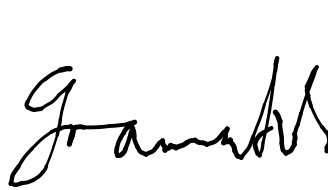
\includegraphics[width=0.35\textwidth]{src/abbildungen/unterschrift}\vspace*{-0.35cm}
		\\
		\rule[0.5ex]{12em}{0.55pt} & \rule[0.5ex]{12em}{0.55pt} \\
		(Ort, Datum) & (Eigenhändige Unterschrift)
		\\
	\end{tabular*} \\\label{tab:unterschriftSperrvermerk}
\end{table}
\newpage


%-----------------------------------
% Glossar
%-----------------------------------

    \printglossaries
    \newpage

%-----------------------------------
% Seitennummerierung auf arabisch und ab 1 beginnend umstellen
%-----------------------------------
    \pagenumbering{arabic}
    \setcounter{page}{1}

%-----------------------------------
% Kapitel / Inhalte
%-----------------------------------
%TC:endignore
% Die Kapitel werden über folgende Datei eingebunden
    % Hinzugefügt aufgrund von Issue 167
%-----------------------------------
% Kapitel / Inhalte
%-----------------------------------
\section{Einleitung}\label{sec:einleitung}

$35$ Jahre nach dem ersten Cyberangriff\autocite[\vglf][]{shackelford-2018} und $24$ Jahre nach dem ersten \ac{ddos}"~Angriff\autocite[\vglf][]{mit-2019} werden regelmäßig neue Sicherheitslücken in Netzwerken und Programmen gefunden und ausgenutzt.
Die Anzahl der Mal- und Ransomware Angriffe sank zwar durch die Coronapandemie ein wenig, war davor jedoch auf einem historischen Maximum.\autocites[][\pagef 21]{statista-malware}[][\pagef 33]{statista-ransomware}
Zudem ist der Anteil der Unternehmen, die von einem Cyberangriff betroffen waren, so hoch wie noch nie.\autocite{statista-share-ransomware}
Auch die schnelle Verbreitung von \ac{iot}"~Geräten erfordert immer stärker das Absichern von Netzwerken, um sowohl die Infrastruktur, als auch den Geräten zugängliche Daten zu schützen.\autocite[\vglf][\pagef 57143]{syed:2022}
So sind viele Unternehmen, besonders solche die auf kritischer Infrastruktur basieren oder mit wichtigen Daten arbeiten, an einem möglichst idealen Schutz gegenüber diesen Angriffen interessiert.



\subsection{Zielsetzung}\label{subsec:zielsetzung}
Diese Seminararbeit untersucht die Auswirkungen einer \ac{zta} auf die Bekämpfung moderner Cyberbedrohungen.
Dabei wird untersucht, wie die Implementierung einer \ac{zta} die Häufigkeit von Cyberangriffen und von diesen verursachten Datenverlusten in Unternehmen beeinflusst.

Die erwarteten Ergebnisse umfassen eine potenzielle Verringerung von Cyberangriffen und Datenverlusten.
Zugleich werden mögliche Einflüsse auf die Benutzerfreundlichkeit und Produktivität der Mitarbeiter untersucht, um einen ausgewogenen Ansatz zwischen Sicherheit und Arbeitsleistung zu finden.

Dabei wird versucht, die Forschungsfrage \enquote{\myForschungsfrage} zu beantworten.

Zur Erstellung der Seminararbeit wird primär Literaturarbeit durchgeführt, welche sich auf eine systematische Analyse und Synthese bestehender wissenschaftlicher Quellen und Publikationen stützt\autocite[\vglf][\pagef 6]{fink-2019}.
Hierzu wird zunächst ausführlich nach bestehender Literatur recherchiert, welche dann nach Relevanz für das Thema selektiert wird.
Anschließend werden die gewählten Quellen sorgfältig gelesen und analysiert.
Die relevanten Informationen dieser werden extrahiert, dies beinhaltet Daten, Fallstudien und Expertenmeinungen.

Die gesammelten Ergebnisse werden darauf in einem ganzheitlichen Ansatz zusammengeführt, um die Forschungsfrage zu beantworten und die zu erwartenden Ergebnisse zu evaluieren.

Die Wahl der methodischen Herangehensweise ermöglicht eine gründliche Untersuchung des Themas, indem sie auf etablierte wissenschaftliche Erkenntnisse und Fachwissen zurückgreift.
Dies gewährleistet eine fundierte und objektive Analyse der Auswirkungen einer Zero"~Trust Netzwerkarchitektur auf moderne Cyberbedrohungen und die Mitarbeitererfahrung.

\subsection{Aufbau der Arbeit}\label{subsec:aufbau-der-arbeit}
\autoref{sec:grundlagen} führt verschiedene Grundlagen für die Ausarbeitung dieser Seminararbeit ein.
Zunächst werden \acp{zta} definiert, sowie die Entwicklung und der historische Hintergrund dieser erklärt.
Darauf werden Prinzipien von \ac{zta} dargestellt und ein Vergleich zu anderen Sicherheitsansätzen gebildet.

\autoref{sec:moderne-cyberbedrohungen} stellt verschiedene Arten von Cyberbedrohungen wie Malware- oder Phishingangriffe dar.
Zudem werden die Trends in der Cyberkriminalität erläutert.

In \autoref{sec:zta-im-detail} wird der Aufbau und die Komponenten von \ac{zta}, sowie die Implementierung dieser in Unternehmen gezeigt.
Außerdem werden Vor- und Nachteile von Zero-Trust gegeneinander aufgewogen.

Zuletzt werden in \autoref{sec:auswirkungen-und-resultate-von-zero-trust} die Auswirkungen auf die Sicherheit von Netzwerken, sowie die Reduzierung der Angriffsfläche erläutert.
Zudem belichtet dieser Abschnitt, wie Zero-Trust sensible Daten schützt, zeigt die Messbarkeit der Auswirkungen auf die Sicherheit und stellt Probleme dar.
\newpage


\section{Grundlagen}\label{sec:grundlagen}
\acp{zta} haben in den letzten Jahren an Bedeutung gewonnen, da traditionelle Sicherheitsansätze immer weniger effektiv gegen moderne Cyberbedrohungen werden.
In einer zunehmend vernetzten und digitalisierten Welt, in der Unternehmensdaten und -ressourcen ständig Bedrohungen ausgesetzt sind, wird die Implementierung einer \ac{zta} zu essenziellen Sicherheitsstrategie.

Dieser Abschnitt widmet sich der eingehenden Analyse von \ac{zta}, einschließlich ihrer historischen Entwicklung sowie den zugrunde liegenden Prinzipien.

\subsection[Definition einer Zero-Trust-Architektur]{Definition einer \ac{zta}}\label{subsec:definition-einer-zta}
\ac{zt} bezeichnet eine Sammlung an Maßnahmen der Cybersicherheit, welche darauf basieren, die Verteidigungen von netzwerkbasierten Umfängen auf Nutzer und Ressourcen umzuleiten\autocite[\vglf][\pagef 4]{NIST:800207}.
Darüber hinaus ist eine \ac{zta} ein Cybersicherheitsplan einer Einrichtung, der die Konzepte von \ac{zt} umsetzt und Zugriffsrichtlinien, Arbeitsabläufe und Beziehungen zwischen Komponenten umfasst\autocite[\vglf][\pagef 4]{NIST:800207}, welche das reduzieren der vergebenen Berechtigungen auf ein Minimum beinhalten.

Das Ziel einer \ac{zta} ist es, \glsdisp{autorisierung}{unautorisierten} Zugriff auf Daten und Leistungen zu verhindern und hierbei das Durchführen der Zugriffskontrollen so detailliert wie möglich zu gestalten.


\subsection{Entwicklung und historischer Hintergrund}\label{subsec:entwicklung-und-historischer-hintergrund}
Zscaler hat im Jahr 2022 die Entwicklung des \ac{zt}-Konzepts knapp zusammengefasst.\autocites[\vglf][]{zscaler-2022b}
Die ersten Grundsteine, die zur Entwicklung des \ac{zt}-Konzepts führten, wurden $1987$ gelegt.
In diesem Jahr wurde von Entwicklern der \ac{dec} eine Studie zum Thema Firewall-Technologie veröffentlicht, wodurch die \enquote{Festung mit Burggraben} als Standardmodell der Netzwerksicherheit etabliert wurde.\autocites[\vglf][]{zscaler-2022b}

Im Jahr $1994$ wurde der Begriff \enquote{\ac{zt}} im Rahmen einer Doktorarbeit über Computersicherheit geprägt.
Der Autor untersuchte Vertrauen als ein mathematisch beschreibbares, endliches Gut.\autocite[\vglf][]{marsh-1994}
Im selben Jahr wurden Firewalls als eine harte Schale um einen weichen Kern, wie bei einem Ei, beschrieben.
Wenn ein Angreifer die Firewall überwinden kann, stünde ihm das ganze Netzwerk zur Verfügung. \autocite[\vglf][\pagef 29]{world-1994}

Die erste Version des 802.1X-Protokolls\autocite[\vglf][]{IEEE-2001} wurde im Jahr $2001$ veröffentlicht und als Standard für Netzzugangskontrollen eingeführt.
In diesem Protokoll wird die Authentifizierung von Netzverbindungen sowie die Vergabe von Zugriffsrechten auf Netzwerkebene vorgesehen.
Dadurch, dass das Protokoll komplexe Vorgänge vorschreibt, war es nicht zur allgemeinen Implementierung geeignet.\autocite[\vglf][]{zscaler-2022b}
Zusätzlich wurde auch in $2001$ die erste Version des \ac{osstmm} mit dem Fokus auf Vertrauen veröffentlicht.\autocite[\vglf][]{osstmm-2001}

Um das Jahr $2007$ wurde die dritte Version des \ac{osstmm} veröffentlicht, welche in einem ganzen Kapitel über die Schwachstelle \enquote{Vertrauen} in Systemen befasst.\autocite[\vglf][]{osstmm-2010}

Eine weitere Prägung des Begriffes \enquote{\ac{zt}} fand im Jahr $2010$ statt, als der Analyst Kindervag in einem Forschungsbeitrag die Verlagerung der Authentifizierung und Cybersicherheit in den Datenpfad vorsieht und auch die Segmentierung zwischen einzelnen Sitzungen fordert.
Weiterhin wird das Paradigma des Netzwerkzugangs verhaftet, der Sicherheitsperimeter wird allerdings ins Netzwerk verschoben.\autocites[\vglf][]{zscaler-2022b}[\vglf][]{kindervag-2010}

$2018$ arbeiteten Forscher von \ac{nist} und \ac{nccoe} zusammen an einem Projekt, welches zur Veröffentlichung der \ac{nist} Leitlinie SP 800--207\autocite{NIST:800207} im Jahr $2020$ als ein erstes einheitliches Framework für \acp{zta} führte.
Diese definiert \ac{zt} als eine Sammlung verschiedener Konzepte und Ideen, welche die Unsicherheit bei anfragenbezogenen Zugriffsentscheidungen in Informationssystemen verringern sollen.
Diese Veröffentlichung leitete einen Paradigmenwechsel ein, da erstmals \ac{zt} nicht mehr im Kontext des Netzwerkzugangs definiert wird.\autocite[\vglf][]{zscaler-2022b}

Im Jahr $2021$ hat das \ac{ncsc} im Vereinigten Königreich empfohlen, dass Netzwerkarchitekten einen \ac{zt} Ansatz für neue IT-Lösungen in Anbetracht nehmen insbesondere wenn signifikante Nutzung von Cloud-Services geplant ist.\autocite{ncsc-2021}
Zusätzlich wurden im Jahr $2022$ alle US-Behörden zur Umstellung auf \ac{zt} bis $2024$ verpflichtet.\autocite[\vglf][]{zscaler-2022b}


\subsection{Prinzipien und Konzepte von Zero-Trust}\label{subsec:prinzipien-und-konzepte-von-zero-trust}
In einem System, welches \ac{zt} implementiert, muss jede Anfrage bevor sie auf die Ressourcen zugreifen kann, in einem \gls{pdp}/\gls{pep} überprüft werden\autocite[\vglf][\pagef 4]{NIST:800207}.

Eine \ac{zta} wird mit dem Gedanken entwickelt und umgesetzt, die folgenden Grundsätze umzusetzen:
\begin{itemize}
    \item Alle Datenquellen und Rechenleistungen werden als Ressourcen angesehen,
    \item Unabhängig der Netzwerkposition ist jegliche Kommunikation gesichert,
    \item Der Zugriff auf einzelne Ressourcen erfolgt auf einer Pro-Sitzung Grundlage,
    \item Zugriff auf Ressourcen wird durch dynamische Regelungen festgelegt und kann von verschiedenen Attributen, wie die Identität des \glspl{client} beeinflusst werden,
    \item Das Unternehmen überwacht und misst die \gls{integritaet} aller eigenen und verbundenen Ressourcen,
    \item Jegliche Ressourcen \gls{authentifizierung} und \gls{autorisierung} ist dynamisch und erzwungen, bevor Zugriff gewährt werden kann,
    \item Das Unternehmen sammelt so viele Informationen über den aktuellen Status der Ressourcen, Netzwerkinfrastruktur und Kommunikationen wie möglich und nutzt diese, um die Sicherheit zu erhöhen.\autocite[\vglf][\pagef 6-7]{NIST:800207}
\end{itemize}

\newpage


\section{Moderne Cyberbedrohungen}\label{sec:moderne-cyberbedrohungen}
%\todo[inline]{Eventuell Einleitungstext schreiben}

\subsection{Trends und Entwicklungen in der Cyberkriminalität}\label{subsec:trends-und-entwicklungen-in-der-cyberkriminalitat}
In den letzten Jahren hat die Anzahl der Cyberkriminalitätsfälle in Deutschland stark zugenommen.
So wurden zwar für das Jahr 2022 ein Rückgang von 6.5\% gegenüber dem Vorjahr an erfassten Fällen aufgezeichnet, jedoch bildet sich in dem Zeitraum von 2012 bis 2022 ein Gesamtwachstum von 112\% an erfassten Cyberkriminalitätsfällen\autocite[\vglf][]{bka-cyberkriminalitaet}.

Analog zu der Anzahl der aufgezeichneten Fälle steigen auch die Kosten, die Cyberkriminalität verursacht, sowie die Ausgaben die für IT-Sicherheit in Deutschland vorgenommen werden stetig.
2018 haben Cyberkriminalitätsvorfälle deutschen Unternehmen durchschnittlich 13,12 Millionen US-Dollar\footnote{Heutiger Wert ungefähr 10,23 Millionen Euro} gekostet, was gegenüber dem Vorjahr ein Zuwachs von fast 18\% darstellt\autocite[\vglf][]{accenture-cyberkrime-kosten}.
2021 wurden so ungefähr 6,9 Milliarden Euro für IT-Sicherheitsmaßnahmen ausgegeben, was einem Zuwachs von fast 22\% gegenüber dem Vorjahr entspricht\autocite[\vglf][]{bitkom-itsicherheit}, davon wurden geschätzt 1,7 Milliarden Euro für Softwarelösungen ausgegeben\autocite[\vglf][]{bitkom-itsicherheit-segment}.

Wie die Kosten und Ausgaben für Cyberkriminalität steigen auch die möglichen Methoden der Angreifer.
\autoref{fig:cybercrime-chart-absolute} zeigt, dass die Anzahl der Fälle von Cyberkriminalität fast stetig zunimmt.

\begin{figure}[htpb]
    \centering
    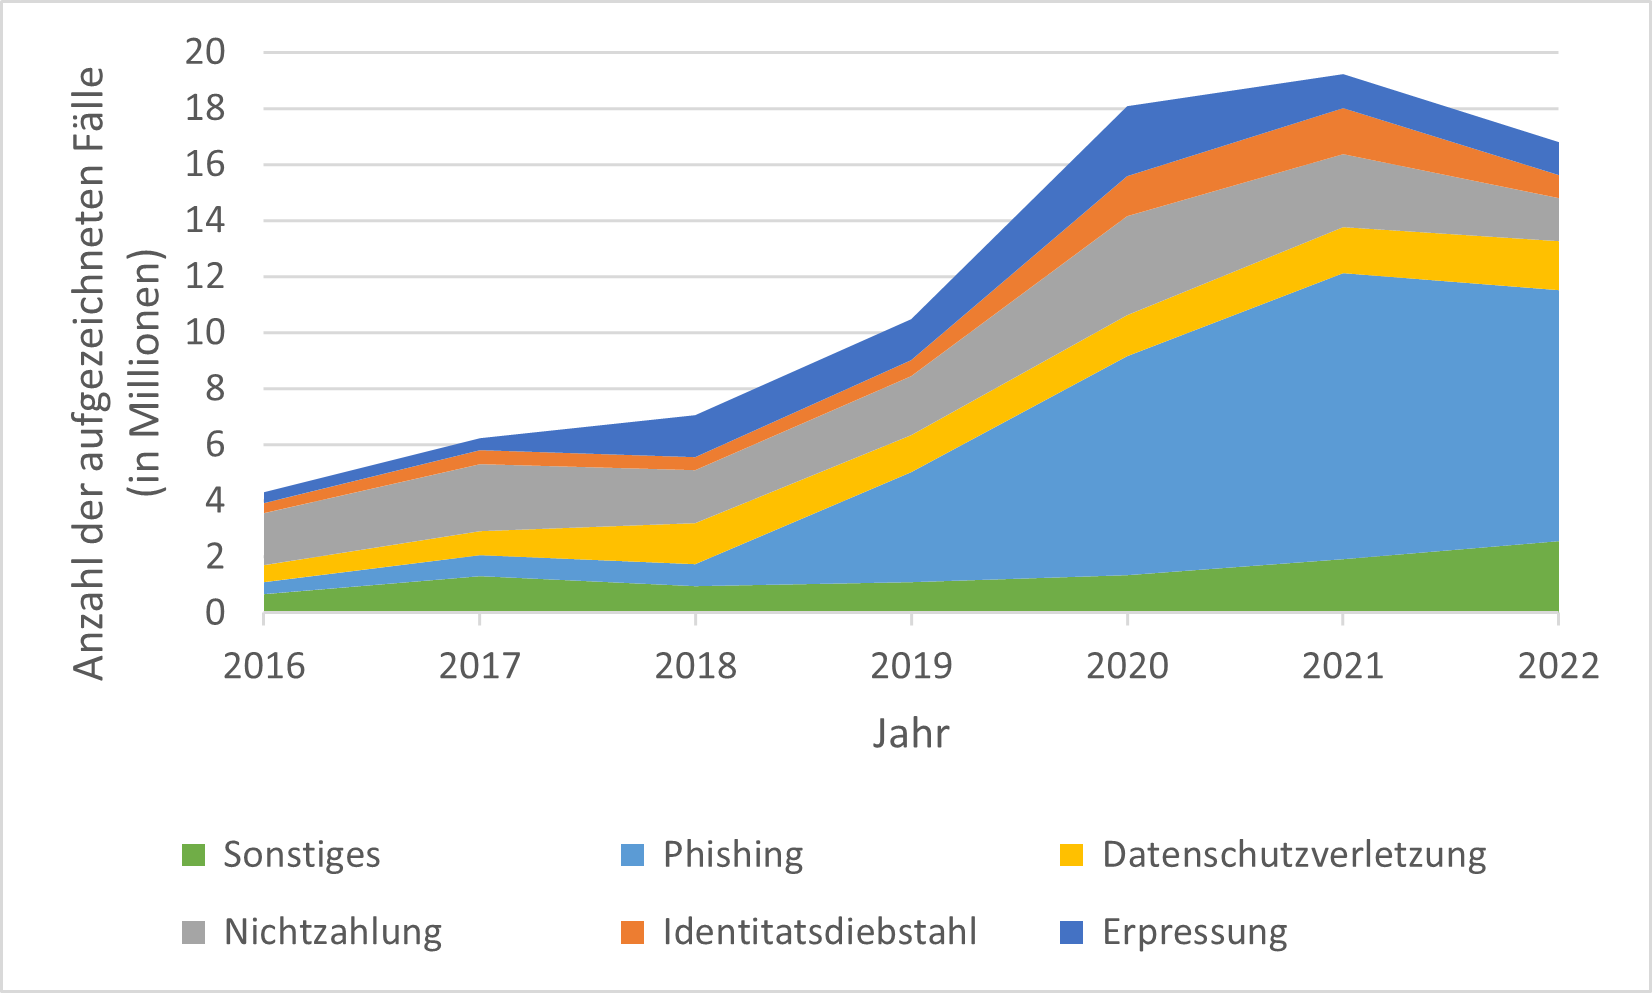
\includegraphics[width = 0.65\linewidth]{src/abbildungen/Aufgezeichnete_Cyberkriminalitaet}
    \captionsetup{width=\linewidth, format=hang}
    \caption[Erfasste Fälle von Cyberkriminalität nach Typ]{Erfasste Fälle von Cyberkriminalität nach Typ.\footnotemark{}\ Stand September 2023}
    \label{fig:cybercrime-chart-absolute}
\end{figure}\ \footnotetext{\cite[\vglf][]{statista-cybersecurity-cybercrime}}

Einzig im Jahr 2022 wurde ein Rückgang der erfassten Fälle aufgezeichnet.
Besonders der Anteil, der Phishingangriffe hat im Vergleich zu 2018 stark zugenommen, wie in \autoref{fig:cybercrime-chart-relative} dargestellt wird.

\begin{figure}[htpb]
    \centering
    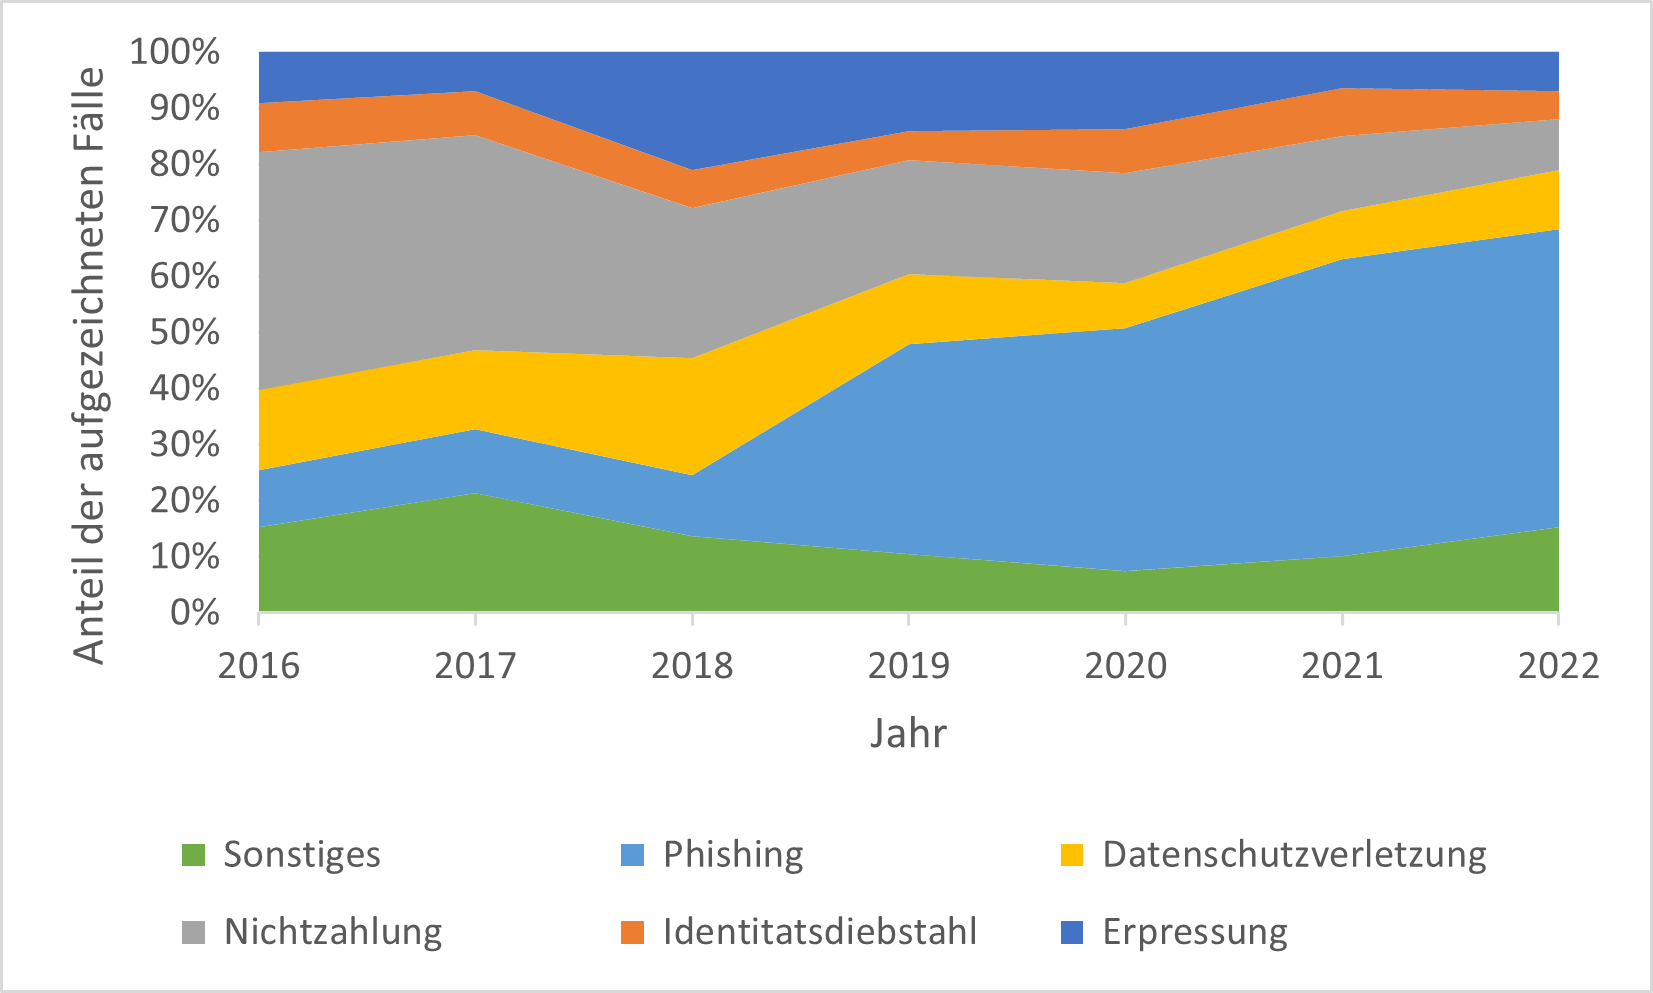
\includegraphics[width = 0.65\linewidth]{src/abbildungen/Anteile_Cyberkriminalitaet}
    \captionsetup{width=\linewidth, format=hang}
    \caption[Anteil einzelner Cyberkriminalitätstypen]{Anteil einzelner Cyberkriminalitätstypen.\footnotemark{}\ Stand September 2023}
    \label{fig:cybercrime-chart-relative}
\end{figure}\ \footnotetext{\cite[\vglf][]{statista-cybersecurity-cybercrime}}
%\todo[inline]{Eventuell Float entfernen, um Fußnote anzupassen!}

\subsection[Arten von Cyberbedrohungen]{Arten von Cyberbedrohungen - Malware, Phishing, DDoS}\label{subsec:arten-von-cyberbedrohungen---malware-phishing-ddos}

Die drei häufigsten Methoden von Cyberattacken sind Malware, Phishing und \ac{ddos} Angriffe.

\begin{definition}
    \label{def:phishing}
    Phishing bezeichnet den Versuch, an vertrauliche Informationen wie Anmeldedaten oder Kreditkarteninformationen zu gelangen, indem ein System innerhalb eines Kommunikationsvorgangs als vertrauenswürdig ausgibt.\autocite[\vglf][\pagef 27]{study-on-phishing-attacks:2018}
\end{definition}

\begin{definition}
    \label{def:malware}
    Malware bezeichnet eine Software, welche ausschließlich Systeme angreift, welche entweder keine anderen Systeme beschädigen, oder welche Malwaresysteme angreifen.\autocite[\vglf][\pagef 108f.]{definition-malware-2010}
\end{definition}

\begin{definition}
    \label{def:ddos}
    Unter \ac{ddos}-Angriffen werden Vorgänge verstanden, gezielt versuchen, ein Netzwerk oder einen Computer die Möglichkeit zu nehmen, gewohnte Dienste auszuführen.
    Bei solchen Angriffen werden die vorhandenen Daten und Systeme weder direkt noch permanent angegriffen, es wird lediglich die Verfügbarkeit dieser Ressourcen unterbunden.\autocite[\vglf][\pagef 190]{ddos-definition-2003}
\end{definition}

Diese Angriffe zielen auf verschiedene Angriffsflächen und haben verschiedene Ziele, welche das korruptieren von Daten oder Systeme oder das Hindern des Zugriffs auf Daten und Systeme beinhalten können.
Um diese Angriffe abzuwehren, gibt es verschiedene Methoden, eine davon ist eine \ac{zta}.


\newpage
\section[Zero-Trust Architektur im Detail]{\ac{zta} im Detail}\label{sec:zta-im-detail}
Da in einer \ac{zta} keinem Gerät und keiner Anwendung vertraut wird, aber alle unterstützt werden, sind verschiedene Maßnahmen notwendig um die erwünschte Sicherheit zu garantieren.
Dies geschieht durch regelmäßiges Überprüfen der \glsdisp{authentifizierung}{Authentizität} und \gls{autorisierung} der Systeme.\autocite[\vglf][\pagef 3]{dsilvia-2021}

\subsection{Komponenten und Aufbau von Zero-Trust}\label{subsec:komponenten-und-aufbau-von-zero-trust}
Jede \ac{zta} wird durch drei Eigenschaften definiert.
Diese stellen sicher, dass (\romannumeral 1) auf alle Ressourcen unabhängig von ihrer physischen oder logischen Position ein sicherer Zugriff erfolgen muss, (\romannumeral 2) strenge Zugriffskontrollmaßnahmen bestehen, und zuletzt (\romannumeral 3) jeglicher Netzwerkverkehr erfasst und aufgezeichnet wird.\autocite[\vglf][\pagef 2]{dsilvia-2021}

\subsubsection{Komponenten einer Zero-Trust Architektur}
Es gibt verschiedene Methoden, eine \ac{zta} einzurichten, von denen viele das Konzept teilen, die Kontrolle nahe an den Anwendungen und Nutzern zu halten anstatt sie in der Netzwerkinfrastruktur auszulagern.\autocite[\vglf][\pagef 4]{buck-2021}
Drei der Grundmethoden einer \ac{zta} sind \glsdisp{authentifizierung}{Anwendungsauthentifizierung}, \glsdisp{authentifizierung}{Gerätauthentifizierung} und Vertrauen, da eine \ac{zta} im Gegensatz zu anderen Sicherheitsinfrastrukturen die \glsdisp{authentifizierung}{Authentizität} regelmäßig überprüft, die Nutzergeräte überprüft und Widersprüchlichkeiten in Anwendungen der Nutzer überwacht und erkennt.\autocite[\vglf][\pagef 3]{dsilvia-2021}

\ac{zt} sollte nicht als einzelne Technologie gesehen werden, sondern stellt durch viele Anforderungen, Kontrollen und Prinzipien einen umfassenden Schutz dar, welcher selbst bei verschwimmender Grenze zwischen Privatem und Arbeit nicht minder wirkt.\autocite[\vglf][Was sind die Komponenten von Zero Trust]{akamai:online}

\subsubsection{Aufbau einer Zero-Trust Architektur}

Eine \ac{zta} lässt jede Anfrage eine Vertrauensevaluation durchgehen.
Eine solche Evaluation kann aus den folgenden, von Horne und Nair dargestellten, Schritten bestehen\autocite[\vglf][\pagef 3]{horne-2021}:
\begin{enumerate}
    \item Vertrauensfaktoren, darunter unter anderem
    \begin{itemize}
        \item \glsdisp{authentifizierung}{Nutzerauthentifizierung},
        \item Nutzerrolle oder -profil,
        \item \glsdisp{authentifizierung}{Gerätauthentifizierung},
        \item Geräteart und -status,
        \item IP-Adresse, \bzw Ort,
        \item Details der Zugriffsanfrage,
        \item Verhaltensdaten,
    \end{itemize}
    \item Vertrauensalgorithmus,
    \item Anforderungen und Anforderungsadministrator, mit den folgenden Richtlinien
    \begin{itemize}
        \item Vertrauensgrenzwerte,
        \item Grundsätze zur Einhaltung der Richtlinien,
        \item Richtlinien für Endgeräte,
        \item Datenschutzrichtlinien
    \end{itemize}
    \item Erlauben oder Ablehnen der Zugriffsanfrage.
\end{enumerate}
Die Überprüfung nach dem $4.$ Schritt der vorherigen Auflistung läuft dabei wie folgt ab:\autocite[\vglf][\pagef 3]{horne-2021}
\begin{enumerate}
    \item Dabei wird die Anfrage zunächst auf die einzelnen Faktoren überprüft und evaluiert.
    \item Anschließend wird aus dem Resultat dieser Evaluation ein Vertrauenswert berechnet, mit welchem die Anfrage überprüft und einzelne Richtlinien zugeschrieben werden.
    \item Zuletzt wird, sofern ein ausreichender Vertrauenswert vorhanden ist, die Anfrage unter Einhaltung der Richtlinien akzeptiert, andernfalls abgelehnt.
\end{enumerate}

\subsection{Implementierung von Zero-Trust in Unternehmen}\label{subsec:implementierung-von-zero-trust-in-unternehmen}
Eine \ac{zta} kann sowohl in einem neuen System implementiert werden, als auch in einem bereits bestehenden eingearbeitet werden.
Hierfür werden die folgenden Annahmen genommen:\autocite[\vglf][\pagef 3]{dsilvia-2021}
\begin{itemize}
    \item Das LAN innerhalb eines Netzwerkes sollte nicht implizit als vertraute Zone behandelt werden.
    \item Mit dem aktuellen Trend, dass in Unternehmen \ac{byod} eingeführt wird, wird davon ausgegangen, dass Geräte, die mit dem Netzwerk verbunden sind, keine Instanz des Unternehmens sind, da jedes Gerät manipuliert werden kann.
    \item Ressourcen sind niemals vertrauenswürdig, \dah vom Standpunkt der Sicherheit aus gesehen muss jede Ressource kontinuierlich bewertet werden und darf nur solange genutzt werden, wie sie benötigt wird.
    \item Cloud-Dienste sind ein wesentlicher Bestandteil jedes Unternehmensnetzwerkes geworden und verdeutlichen, dass nicht alle Unternehmensressourcen innerhalb der Unternehmensinfrastruktur liegen.
    \item Alle Verbindungsanfragen von außerhalb des Unternehmens, wie \zb Remote Desktop, müssen \glsdisp{autorisierung}{autorisiert} und \glsdisp{authentifizierung}{authentifiziert} werden.
    Alle Daten müssen mit \gls{respekt}, \gls{vertraulichkeit}, \gls{integritaet} und \glsdisp{authentifizierung}{Quellenauthentifizierung} übertragen werden.
    \item Ausgehend der obigen Annahmen ist es essenziell, dass alle Ressourcen und Kommunikation zwischen dem Unternehmen und externer Infrastruktur einer ständigen Sicherheitsstrategie unterliegen müssen.
\end{itemize}

\subsection{Vor- und Nachteile von Zero-Trust}\label{subsec:vor-und-nachteile-von-zero-trust}
Eine \ac{zta} bietet verschiedenste Vor- und Nachteile, angefangen von den verbesserten Sicherheitsmetriken, endend bei einer komplexeren Infrastruktur.
Dieser Abschnitt listet und erläutert einzelne dieser Eigenschaften.

\subsubsection{Vorteile}\label{subsubsec:vorteile}
Bei erfolgreicher Implementierung einer \ac{zta} hat jeder Teil des Netzwerkes nur für ein Minimum der Zeit Zugriff auf das Minimum der erforderten Ressourcen.
Dies sorgt dafür, dass ein nahezu umfassender Schutz vor Angriffen besteht, welche besonders Sicherheitslücken in Systemen, die durch, beabsichtigte oder unbeabsichtigte, Vertrauensbrüche entstehen, abzielen\autocite[\vglf][\pagef 146]{Edo-2022}.
Zudem ist eine \ac{zta} flexibler, was die Nutzung von Anwendungen und Geräten betrifft, da die Sicherheitsarchitektur sich nicht auf einzelne Perimeter verlassen muss.\autocites[\vglf][\pagef 28]{shore-2021}[\vglf][]{hunter-2020}
Gleichermaßen stellt eine \ac{zta} eine bessere Einsicht in den Netzverkehr und das Nutzerverhalten dar, was es erneut vereinfacht, Risiken zu erkennen und auf diese zu reagieren.\autocite[\vglf][\pagef 28]{shore-2021}

Besonders Unternehmen, welche ihre Ressourcen primär in Cloud-Systemen verwalten werden einfachere Prozesse in der Umwandlung auf eine \ac{zta} haben, da die Sicherheitsprotokolle bei diesen Systemen meist flexibler einzurichten sind.
Zudem ist eine \ac{zta} in digitalen Unternehmen sehr effektiv, da solche keine klare Perimetergrenze haben, sondern überall existieren wo Kunden, Mitarbeiter oder Partner mit den Diensten interagieren und Daten genutzt werden.
Hierdurch ist eine auf Perimeter basierende Sicherheitsstrategie nicht ausreichend.
Eine \ac{zta} hingegen ermöglicht es, neue Services schnell zu unterstützen, ohne dass eine Verbindung zum gesamten Unternehmesnetzwerk geöffnet wird.
Dies ermöglicht es den Sicherheitsabteilungen an der digitalen Transformation teilzuhaben, anstatt ausschließlich als Verwalter wahrgenommen zu werden.\autocite[\vglf][\pagef 11]{cunningham-2019}

Zusätzlich reduziert eine \ac{zta} die Managementkosten, indem Anzahl und Arten von Sicherheitskontrollen verringert und somit die Anzahl der Managementkonsolen im System reduziert werden.
Dies führt zu einer effizienteren Nutzung von Ressourcen und ermöglicht es den Sicherheitsmitarbeitern in einem Unternehmen, mehr Zeit für substantielle Sicherheitsaktivitäten aufzuwenden.\autocite[\vglf][\pagef 8]{cunningham-2019}

\subsubsection{Nachteile}\label{subsubsec:nachteile}
Während die Vorteile primär auf der technischen Seite einer \ac{zta} liegen, existieren auch Nachteile, welche auf physischer Ebene Auswirkungen zeigen.
So kann sich das Einrichten einer \ac{zta} durch das Erwerben neuer, notwendiger Werkzeuge und Technologien als kostenintensiv darstellen.\autocite[\vglf][\pagef 33]{shore-2021}
Zudem kann die Nutzererfahrung mit dem System geringwertiger als gewünscht ausfallen, da jede Anfrage eine neue \gls{autorisierung} und \glsdisp{authentifizierung}{Authentifizierung} erfordert, was besonders zu Anfängen eine nicht vernachlässigbare Zeitdauer in Anspruch nehmen kann.\autocite[\vglf][\pagef 28]{shore-2021}

Darüber hinaus kann die Implementierung einer \ac{zta} selbst komplex und zeitaufwendig sein, sowie signifikante Änderungen in bestehenden Netzwerkinfrastrukturen und Sicherheitsmaßnahmen erfordern.\autocites[\vglf][\pagef 33]{shore-2021}[\vglf][\pagef 11]{buck-2021}
\newpage


\section{Auswirkungen und Resultate von Zero-Trust}\label{sec:auswirkungen-und-resultate-von-zero-trust}

\subsection{Verbesserung der Sicherheitsebene}\label{subsec:verbesserung-der-sicherheitsebene}
Eine \ac{zta} trägt zur Verbesserung der Sicherheitsebene von Systemen bei, indem es einen Paradigmenwechsel in der Cybersicherheit darstellt.
Das Vertrauen in Personen, Geräte und Prozesse wird zuvor bereits dargestellt auf ein Minimum reduziert, wodurch die Sicherheit erhöht wird.

Die kontinuierliche Überwachung des Datenverkehrs ermöglicht es, sowohl verdächtige Verhaltensweisen und Angriffe schneller zu erkennen und zu unterbinden, als auch aus vergangenen Vorfällen Fehler zu erkennen und die bestehenden Sicherheitsmaßnahmen entsprechend anzupassen.\autocite[\vglf][\pagef 4]{buck-2021}
Durch Mikrosegmentierung, dem Aufteilen eines Netzwerkes in kleinere Segmente, und dem Gewähren von Zugriff ausschließlich auf die für die Anfrage benötigten Ressourcen wird sichergestellt, dass kein überflüssiger und ungewollter Datenverkehr durchgeführt wird.\autocite[\vglf][\pagef 30]{shore-2021}
Hierdurch wird die Anzahl der möglichen ausnutzbaren Lücken im System reduziert.


\subsection{Reduzierung von Angriffsflächen}\label{subsec:reduzierung-von-angriffsflachen}
Durch die Mikrosegmentierung eines Netzwerks mit einer \ac{zta} in kleinere, isolierte Segmente werden Angriffe auf das Segment begrenzt, in dem sie stattfinden, ohne sich auf andere Segmente ausbreiten zu können.
Dies reduziert das Risiko von Datenlecks und unbefugtem Zugriff.\autocites[\vglf][\pagef 20]{shore-2021}[\vglf][\pagef 4]{buck-2021}
Besonders gegen \ac{ddos}-Angrife bietet eine \ac{zta} starken Schutz, da die meist automatisierten Angriffe durch die Mikrosegmentierung nur geringe Bereiche des Systems anwählen können.\autocite[\vglf][\pagef 289]{Eidle-2017}

Des Weiteren trägt die Verwendung von \ac{sdp} dazu bei, dass eine \enquote{Black Box} gebildet wird, welche die Infrastruktur und Ressourcen vor öffentlichem Zugriff verbirgt\autocites[\vglf][\pagef 4]{buck-2021}[\vglf][\pagef 1]{kumar-2019}

\subsection{Schutz sensibler Daten}\label{subsec:schutz-sensibler-daten}
Um eine \ac{zta} einzurichten werden im Allgemeinen fünf Schritte vorausgesetzt.
Diese sind (\lowerromannumeral{1}) das Identifizieren der sensiblen Daten, (\lowerromannumeral{2}) das Erfassen des Datenflusses der sensiblen Daten, (\lowerromannumeral{3}) der Entwurf der \ac{zt}-Parametern, (\lowerromannumeral{4}) das kontinuierliche Überwachen des Systems mit Sicherheitsanalysen und (\lowerromannumeral{5}) das Einführen der Steuerung und Automatisierung der Sicherheitsmaßnahmen.\autocites[\vglf][\pagef 2-3]{ahmed-2020}[\vglf][]{balaouras-2023}

\subsection{Probleme}\label{subsec:probleme}
\newpage
\section{Fazit}\label{sec:fazit}

Mit dieser Seminararbeit sollten die Auswirkungen einer \ac{zta} auf die Sicherheit eines Systems, sowie auf den Datenverlust dargestellt werden.
Mithilfe einer ausführlichen Analyse der existierenden Literatur wurden diese Auswirkungen veranschaulicht.
Des Weiteren bietet diese Arbeit eine ausführliche Einführung in das Thema \ac{zt} und stellt den Aufbau einer \ac{zta} dar.

Die Analyse der bestehenden Literatur zeigte, dass eine \ac{zta} in verschiedenen Unternehmen weltweit bereits genutzt wird und die Auswirkungen dieser messbar sind.
Besonders im Verwaltungsbereich auf Bundesebene sind \acp{zta} verbreitet, wie in \autoref{subsec:entwicklung-und-historischer-hintergrund} dargestellt wurde.

Die zentralen Auswirkungen einer \ac{zta}, sowie das Potenzial in der weiteren Verbreitung dieser, sind eine Verringerung der Häufigkeit von Cyberangriffen und damit verbundenen Datenverlusten in Unternehmen.
Dies wird durch die strikte Überprüfung von Netzwerkzugriffen bereitgestellt, wodurch eine \ac{zta} eine robuste Sicherheitslösung darstellt.
Dabei muss jedoch beachtet werden, dass eine \ac{zta} einen Einschnitt in die Benutzerfreundlichkeit und Geschwindigkeit des Systems darstellt, da für die Überprüfungen verschiedene Daten eingegeben, gesammelt und gespeichert werden müssen.
Dies stellte im Jahr 2023 für ungefähr ein Drittel der Unternehmen eine Herausforderung beim Aufbau einer \ac{zta} dar, wie in \autoref{fig:zero-trust-challenges} dargestellt.

Zusammenfassend lässt sich jedoch sagen, dass eine \ac{zta} eine positive Wirkung auf die Sicherheit in einem System hat, auch wenn Einbußen in Nutzerfreundlichkeit und Produktivität betrachtet werden.
Damit diese zusätzlich auf einem gleichen Niveau wie vor der Einführung bleiben, müssen weiterführende Maßnahmen getroffen werden.

\ac{zt} ist zwar ein vergleichsweise altes Konzept, die Grundlagen dafür wurden bereits in den 1990er Jahren gelegt, große Verbreitung erfährt das Konzept jedoch erst seit ein paar Jahren.
Besonders Kindervag, \ac{nist} und \ac{ncsc} trugen stark zur Verbreitung und Forschung an \ac{zt} bei, sodass es heute fast ein fertiges Konzept ist, das Unternehmen nur noch implementieren müssen.\autocites{kindervag-2010}{NIST:800207}{ncsc-2021}

Die vorliegende Seminararbeit hat ausschließlich die direkten Auswirkungen einer \ac{zta}, sowie den grundlegenden Aufbau einer solchen betrachtet.
In einer tiefergehenden Betrachtung kann es daher sinnvoll sein, die Interaktionen einer \ac{zta} in Kombination mit anderen Sicherheitsmaßnahmen zu untersuchen.

%TC:ignore

%-----------------------------------
% Apendix / Anhang
%-----------------------------------
%\newpage
%\section*{\AppendixName} %Überschrift "Anhang", ohne Nummerierung
%\addcontentsline{toc}{section}{\AppendixName} %Den Anhang ohne Nummer zum Inhaltsverzeichnis hinzufügen

%\begin{appendices}
% Nachfolgende Änderungen erfolgten aufgrund von Issue 163
%%\makeatletter
%\renewcommand\@seccntformat[1]{\csname the#1\endcsname:\quad}
%\makeatother
%\addtocontents{toc}{\protect\setcounter{tocdepth}{0}} %
%	\renewcommand{\thesection}{\AppendixName\ \arabic{section}}
%	\renewcommand\thesubsection{\AppendixName\ \arabic{section}.\arabic{subsection}}
%	    
%\end{appendices}
%\addtocontents{toc}{\protect\setcounter{tocdepth}{2}}

%-----------------------------------
% Literaturverzeichnis
%-----------------------------------
    \newpage

    \printbibliography[nottype=online,heading=bibintoc,title={Literaturverzeichnis}]
    \newpage
    \printbibliography[type=online,heading=subbibliography,title={\headingNameInternetSources}]

% neue Seite für Internetquellen-Verzeichnis
%\newpage


%\printbibliography[nottype=online, nottype=standard, nottype = patent,heading=bibintoc,title={Literaturverzeichnis}]
%\printbibliography[type=online,heading=subbibliography,title={\headingNameInternetSources}]
%\printbibliography[filter = standards, heading = subbibliography, title = {Standardsverzeichnis}]

%    \newpage\renewcommand{\indexname}{Stichwortverzeichnis}
%    \addcontentsline{toc}{section}{Stichwortverzeichnis}
%    \printindex

    %TC:ignore
\newpage
\pagenumbering{gobble} % Keine Seitenzahlen mehr

%-----------------------------------
% Ehrenwörtliche Erklärung
%-----------------------------------
\section*{Ehrenwörtliche Erklärung}
Hiermit versichere ich, dass die vorliegende Arbeit von mir selbstständig und ohne unerlaubte Hilfe angefertigt worden ist, insbesondere dass ich alle Stellen, die wörtlich oder annähernd wörtlich aus Veröffentlichungen entnommen sind, durch Zitate als solche gekennzeichnet habe.
Ich versichere auch, dass die von mir eingereichte schriftliche Version mit der digitalen Version übereinstimmt.
Weiterhin erkläre ich, dass die Arbeit in gleicher oder ähnlicher Form noch keiner Prüfungsbehörde/Prüfungsstelle vorgelegen hat.
Ich erkläre mich damit nicht einverstanden, dass die Arbeit der Öffentlichkeit zugänglich gemacht wird.
Ich erkläre mich damit einverstanden, dass die Digitalversion dieser Arbeit zwecks Plagiatsprüfung auf die Server externer Anbieter hochgeladen werden darf.
Die Plagiatsprüfung stellt keine Zurverfügungstellung für die Öffentlichkeit dar.



\par\medskip
\par\medskip

\vspace{5cm}

\begin{table}[H]
	\centering
	\begin{tabular*}{\textwidth}{c @{\extracolsep{\fill}} ccccc}
		\myOrt, \the\day.\the\month.\the\year
		&
		% Hinterlege deine eingescannte Unterschrift im Verzeichnis /abbildungen und nenne sie unterschrift.png
		% Bilder mit transparentem Hintergrund können teils zu Problemen führen
		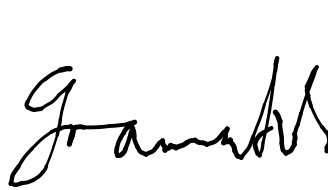
\includegraphics[width=0.35\textwidth]{src/abbildungen/unterschrift}\vspace*{-0.35cm}
		\\
		\rule[0.5ex]{12em}{0.55pt} & \rule[0.5ex]{12em}{0.55pt} \\
		(Ort, Datum) & (Eigenhändige Unterschrift)
		\\
	\end{tabular*} \\\label{tab:unterschrift}
\end{table}
%TC:endignore
%TC:endignore
\end{document}
